\chapter{Form factors} \label{appendixff}

The form factors of the following shapes have been implemented in \BornAgain\ :
\begin{itemize}
\item Parallelepiped, \SecRef{Parallelepiped}  
\item Box, \SecRef{Box} 
\item Prism3, \SecRef{Prism3}  
\item Tetrahedron, \SecRef{Tetrahedron} 
\item Prism6, \SecRef{Prism6}  
\item Cone6, \SecRef{Cone6} 
\item Pyramid, \SecRef{Pyramid} 
\item Anisotropic pyramid, \SecRef{AnisoPyramid} 
\item Cuboctahedron, \SecRef{Cuboctahedron}  
\item Cylinder, \SecRef{Cylinder} 
\item Ellipsoidal cylinder, \SecRef{EllipsoidalCylinder} 
\item Cone, \SecRef{Cone} 
\item Full sphere, \SecRef{FullSphere} 
\item Truncated sphere, \SecRef{Sphere} 
\item Full spheroid, \SecRef{FullSpheroid}  
\item Truncated spheroid. \SecRef{Spheroid} 
\item Hemi-ellipsoid, \SecRef{HemiEllipsoid}  
\item Ripple1, \SecRef{Ripple1}  
\item Ripple2, \SecRef{Ripple2}  
\end{itemize}

In \BornAgain\ the form factor is defined as
\begin{equation*}
F(\mathbf{q})=\int_V \exp (i\mathbf{q}.\mathbf{r}) d^3 \mathbf{r},
\end{equation*}
where $V$ is the volume of the particle's shape,
$\mathbf{q}=\mathbf{k}_i - \mathbf{k}_f$ is the scattering vector with
$\mathbf{k}_f$ and $\mathbf{k}_i$ the scattered and incident wave
vector, respectively.\\

The particle's shape is parametrized in a cartesian frame, with its
$z$-axis pointing upwards and its origin at the center of the bottom
of the particle: $\mathbf{r}=(x,y,z)$. In the followings, a schematic view will depict this layout for each
form factor.\\


All form factors have been implemented with complex scattering vectors
in order to take any material absorption into account.\\


The particles can be rotated in a different direction by using one of
the following tranformations: \Code{CreateRotateX($\theta$),
  CreateRotateY($\theta$), CreateRotateZ($\theta$)}, where $\theta$ is the
angle of rotation considered from... and capital X, Y, Z mark rotations
around the associated axis. For example, in order to rotate a pyramid by $45^{\circ}$ around
$z$-axis, the user could use the following \Code{Python}\ script:\\

\begin{lstlisting}[language=python, style=eclipseboxed,numbers=none,nolol]
    pyramid_ff = FormFactorPyramid(10*nanometer, 5*nanometer, deg2rad(54.73 ) )
    pyramid = Particle(m_particle, pyramid_ff)
    angle_around_z = 45.*degree
    transform = Transform3D.createRotateZ(angle_around_z)
    particle_decoration = ParticleDecoration()
    particle_decoration.addParticle(pyramid, transform) 
\end{lstlisting}

\newpage
%%%%%%%%%%%%%%%%%%%%%%%%%%%%%%%%%%%%
\section{Parallelepiped} \SecLabel{Parallelepiped}  

\subsection{Real-space geometry}
It is a square cuboid (see fig.~\ref{parallelepiped}.

\begin{figure}[ht]
\begin{center}
%\includegraphics[width=0.6\columnwidth]{Figures/Parallelepiped}
\caption{Sketch of a Parallelepiped.}
\end{center}
\label{parallelepiped}
\end{figure}

\paragraph{Parameters:}
\begin{itemize}
\item length of one side of the square base $L$,
\item height $H$.
\end{itemize}

\paragraph{Properties:}
\begin{itemize}
\item volume $V= L^2 H$,
\item particle surface seen from above $S =L^2$.
%\item radius of gyration. 
\end{itemize}

\subsection{Expression of the form factor}
\begin{equation*}
F_{\rm{Parallelepiped}}(\mathbf{q},L, H) = L^2 H\exp(i q_z \frac{H}{2}) \sinc(q_x\frac{L}{2})
\sinc(q_y\frac{L}{2})\sinc(q_z \frac{H}{2}).
\end{equation*}

\paragraph{Syntax:} \Code{FormFactorParallelepiped(length, height)}

\subsection{Examples}
Figure~\ref{figFFparallelEx} shows the normalized intensity
$|F|^2/V^2$, computed with $L=10$~nm and $H=13$~nm.
\begin{figure}[h]
\begin{center}
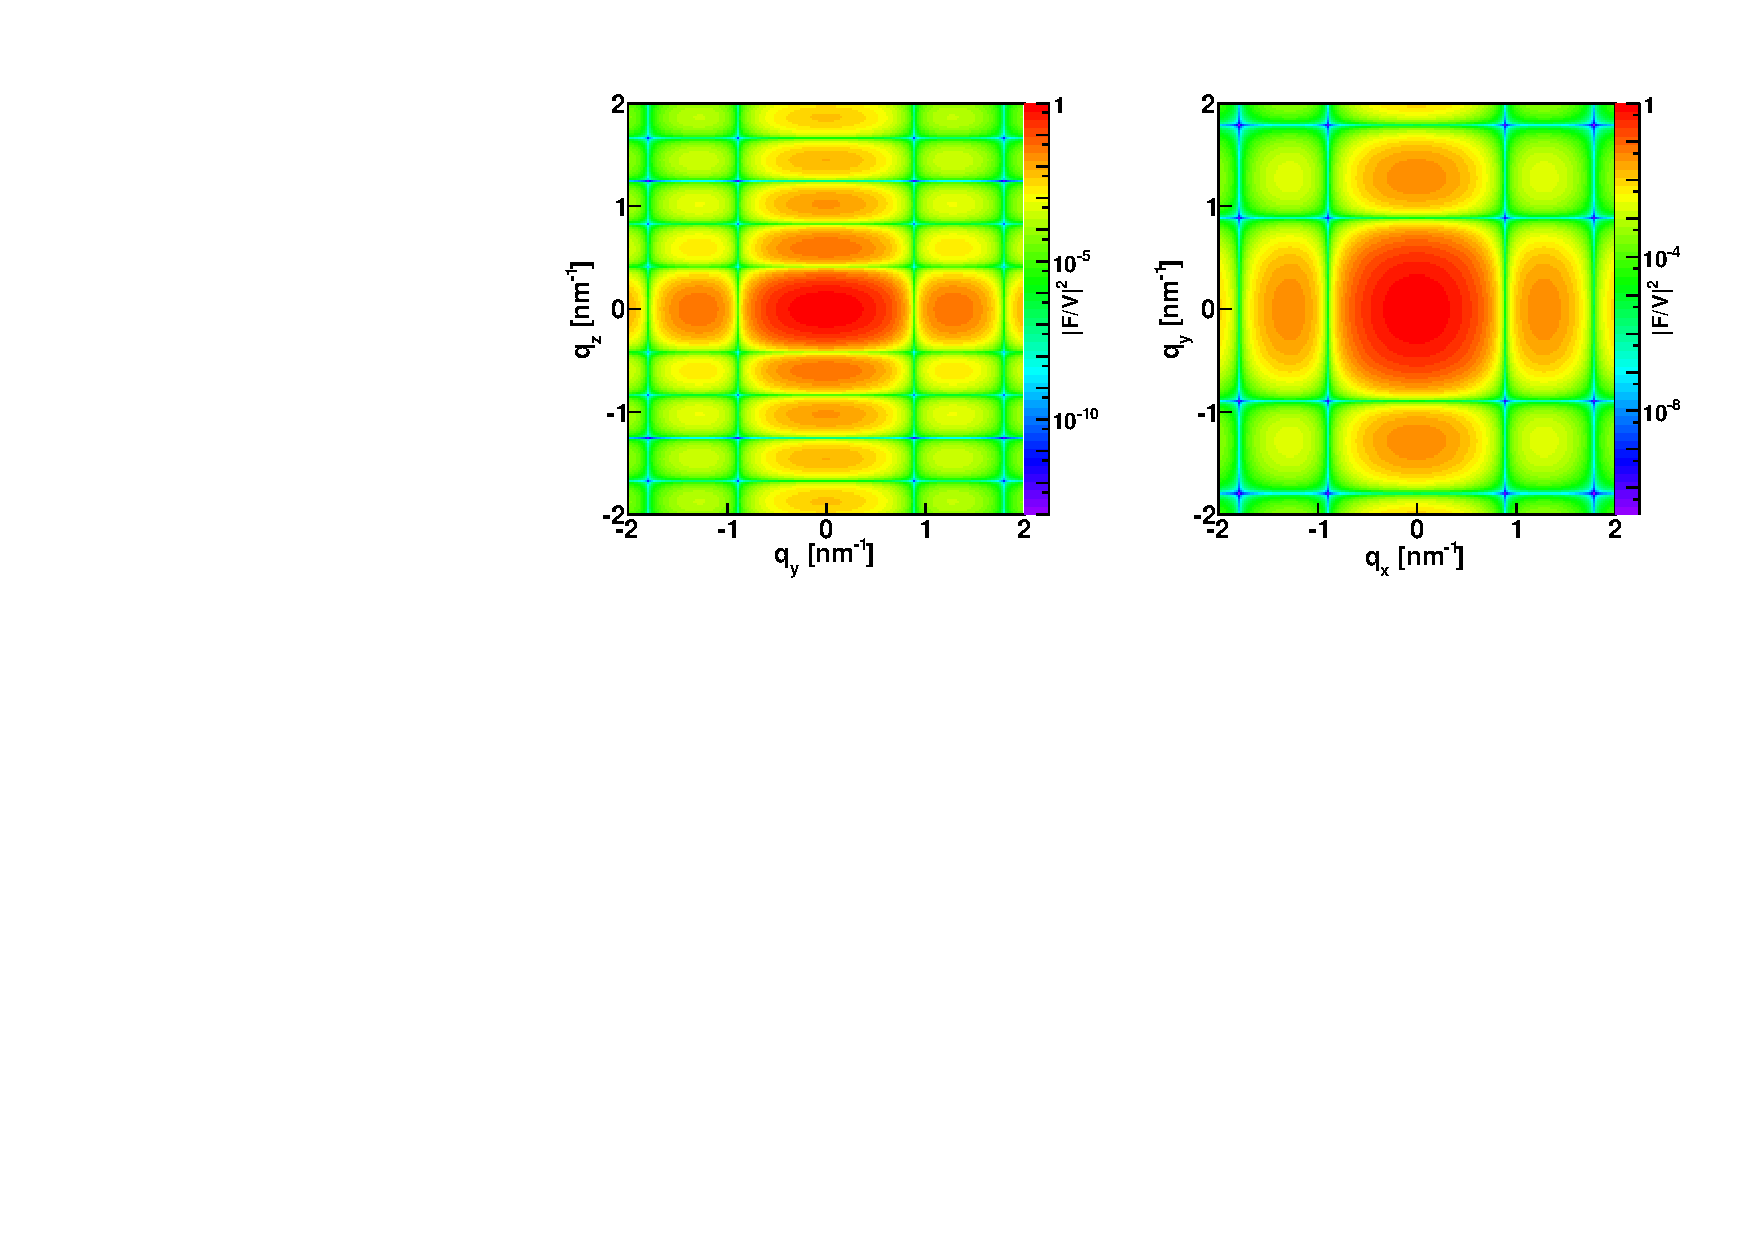
\includegraphics[width=0.9\textwidth]{Figures/figffparallel}
\end{center}
\caption{Normalized intensity for the form factor of a Parallelepiped
  $|F|^2/V^2$, plotted against ($q_z$, $q_y$) and  ($q_x$, $q_y$) and computed with $L=10$~nm and $H=13$~nm.}
\label{figFFparallelEx}
\end{figure}

%\subsection{Parameter dependence}
%Figures~\ref{figFFParallelpardeph} and \ref{figFFParallelpardepr} show the normalized intensity
%$|F|^2/V^2$, computed with [$L=8$~nm and $H=4$, 5 and 6~nm] and [$H=6$~nm and $L=4$,6, and 8~nm:], respectively.
%\begin{figure}[h]
%\begin{center}
%\includegraphics[width=0.9\textwidth]{Figures/ffparallelpardeph}
%\end{center}
%\caption{Normalized intensity for the form factor of a Parallelepiped
%  $|F|^2/V^2$, computed with $L=8$~nm and different values of $H$.}
%\label{figFFParallelpardeph}
%\end{figure}

%\begin{figure}[h]
%\begin{center}
%\includegraphics[width=0.9\textwidth]{Figures/ffparallelpardepr}
%\end{center}
%\caption{Normalized intensity for the form factor of a Parallelepiped $|F|^2/V^2$, computed with $H=6$~nm and different values of $R$.}
%\label{figFFParallelpardepr}
%\end{figure}
%\FloatBarrier


%\subsection{Related particle shapes}
%\begin{itemize}
%\item Box~(\SecRef{Box}),
%\item Prism3~(\SecRef{Prism3}), 
%\item Prism6~(\SecRef{Prism6}),  
%\item Pyramid~(\SecRef{Pyramid}).
%\end{itemize}

\subsection{References}
The parameters characterizing a Parallelepiped are different from
those used in \Code{IsGISAXS}. We use the full side length of the
square base: $L= 2 R_{\rm{\Code{IsGISAXS}}}$.
\newpage{\cleardoublepage}
%%%%%%%%%%%%%%%%%%%%%%%%%%%%%%%%%%%%
\section{Box} \SecLabel{Box} 

\subsection{Real-space geometry}
This shape is a rectangular cuboid or a right rectangular prism as
shown in fig.~\ref{box}. 

\begin{figure}[ht]
\begin{center}
%\includegraphics[width=0.6\columnwidth]{Figures/Drawing5}
\caption{Sketch of a Box.}
\end{center}
\label{box}
\end{figure}


\paragraph{Parameters:}
\begin{itemize}
\item length of the base $L$,
\item width of the base $W$,
\item height  $H$.
\end{itemize}

\paragraph{Properties:}
\begin{itemize}
\item volume $V= LWH$,
\item particle surface seen from above $S = LW$.
%\item radius of gyration
\end{itemize}

\subsection{Expression of the form factor}

\begin{equation*}
F_{\rm{Box}}(\mathbf{q},L,W,H)= L W H\exp(i q_z \frac{H}{2}) \sinc(q_x \frac{L}{2})
\sinc(q_y \frac{W}{2}) \sinc(q_z \frac{H}{2})
\end{equation*}
    
where $\sinc(x)=\sin(x)/x$ is the cardinal sine.

\paragraph{Syntax:} \Code{FormFactorBox(length, width, height)}

\subsection{Examples}
Figure~\ref{figFFBoxEx} shows the normalized intensity
$|F|^2/V^2$, computed with $L=20$~nm, $W=16$~nm, $H=13$~nm, and
$\alpha=60^{\circ}$:

\begin{figure}[h]
\begin{center}
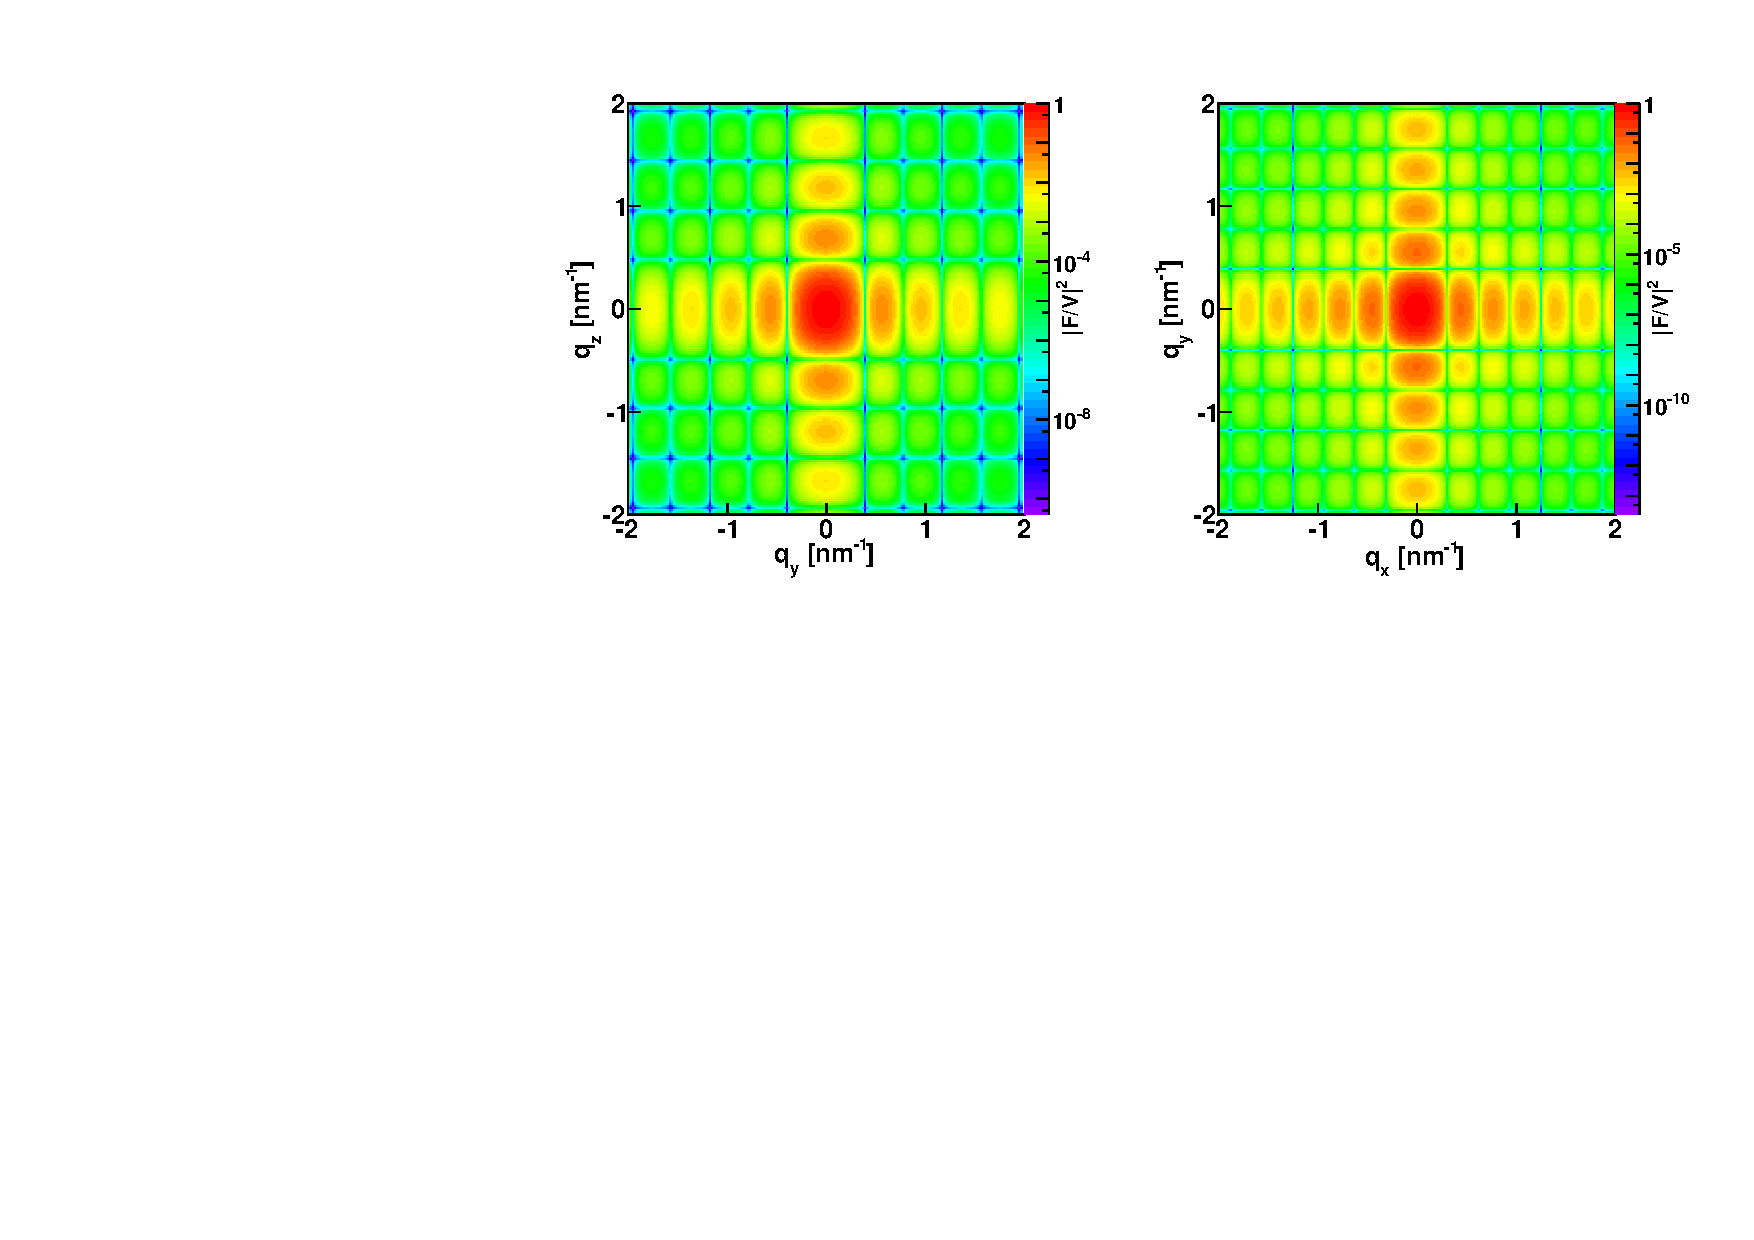
\includegraphics[width=0.9\textwidth]{Figures/figffbox}
\end{center}
\caption{Normalized intensity for the form factor of a Box
  $|F|^2/V^2$, plotted against ($q_z$, $q_y$) and  ($q_x$, $q_y$) and computed with $L=20$~nm, $W=16$~nm, and $H=13$~nm.}
\label{figFFBoxEx}
\end{figure}

\FloatBarrier

\subsection{References}
\BornAgain\ uses a different convention for the parameters in comparison with \Code{IsGISAXS}, where the half length
values are used (see fig.~\ref{box}).

\newpage{\cleardoublepage}
%%%%%%%%%%%%%%%%%%%%%%%%%%%%%%%%%%%%
\section{Prism3} \SecLabel{Prism3}
 
\subsection{Real-space geometry}
This shape is a triangular prism, whose base is an equilateral
triangle as shown in fig.~\ref{prism3}.

\begin{figure}[ht]
\begin{center}
%\includegraphics[width=0.6\columnwidth]{Figures/Prism3}
\caption{Sketch of a Prism3.}
\end{center}
\label{prism3}
\end{figure}

\paragraph{Parameters:}
\begin{itemize}
\item length $L$ of one side of the base, 
\item height $H$.
\end{itemize}

\paragraph{Properties:}
\begin{itemize}
\item volume $V= \dfrac{\sqrt{3}}{4} H L^2$,
\item particle surface seen from above $S =\dfrac{\sqrt{3}}{4}L^2$.
%\item radius of gyration.
\end{itemize}

\subsection{Expression of the form factor}
\begin{align*}
F_{\rm{Prism3}}(\mathbf{q},L, H) &= \frac{2 \sqrt{3}}{q_x^2-3q_y^2} \exp(-i \frac{q_y
      L}{2\sqrt{3}})\Big[\exp(i \sqrt{3} q_y L/2 )
    -\cos(q_x L/2)-i \sqrt{3} q_y L/2 \sinc(q_x L/2) \Big] \\
   &\times  H \sinc(q_z H/2 ) \exp(i q_z H/2),
\end{align*}
where $\sinc(x)=\sin(x)/x$ is the cardinal sine.


\paragraph{Syntax:}  \Code{FormFactorPrism3(length, height)}

\subsection{Examples}
Figure~\ref{figFFprism3Ex} shows the normalized intensity
$|F|^2/V^2$, computed with $L=10$~nm and $H=13$~nm.
\begin{figure}[h]
\begin{center}
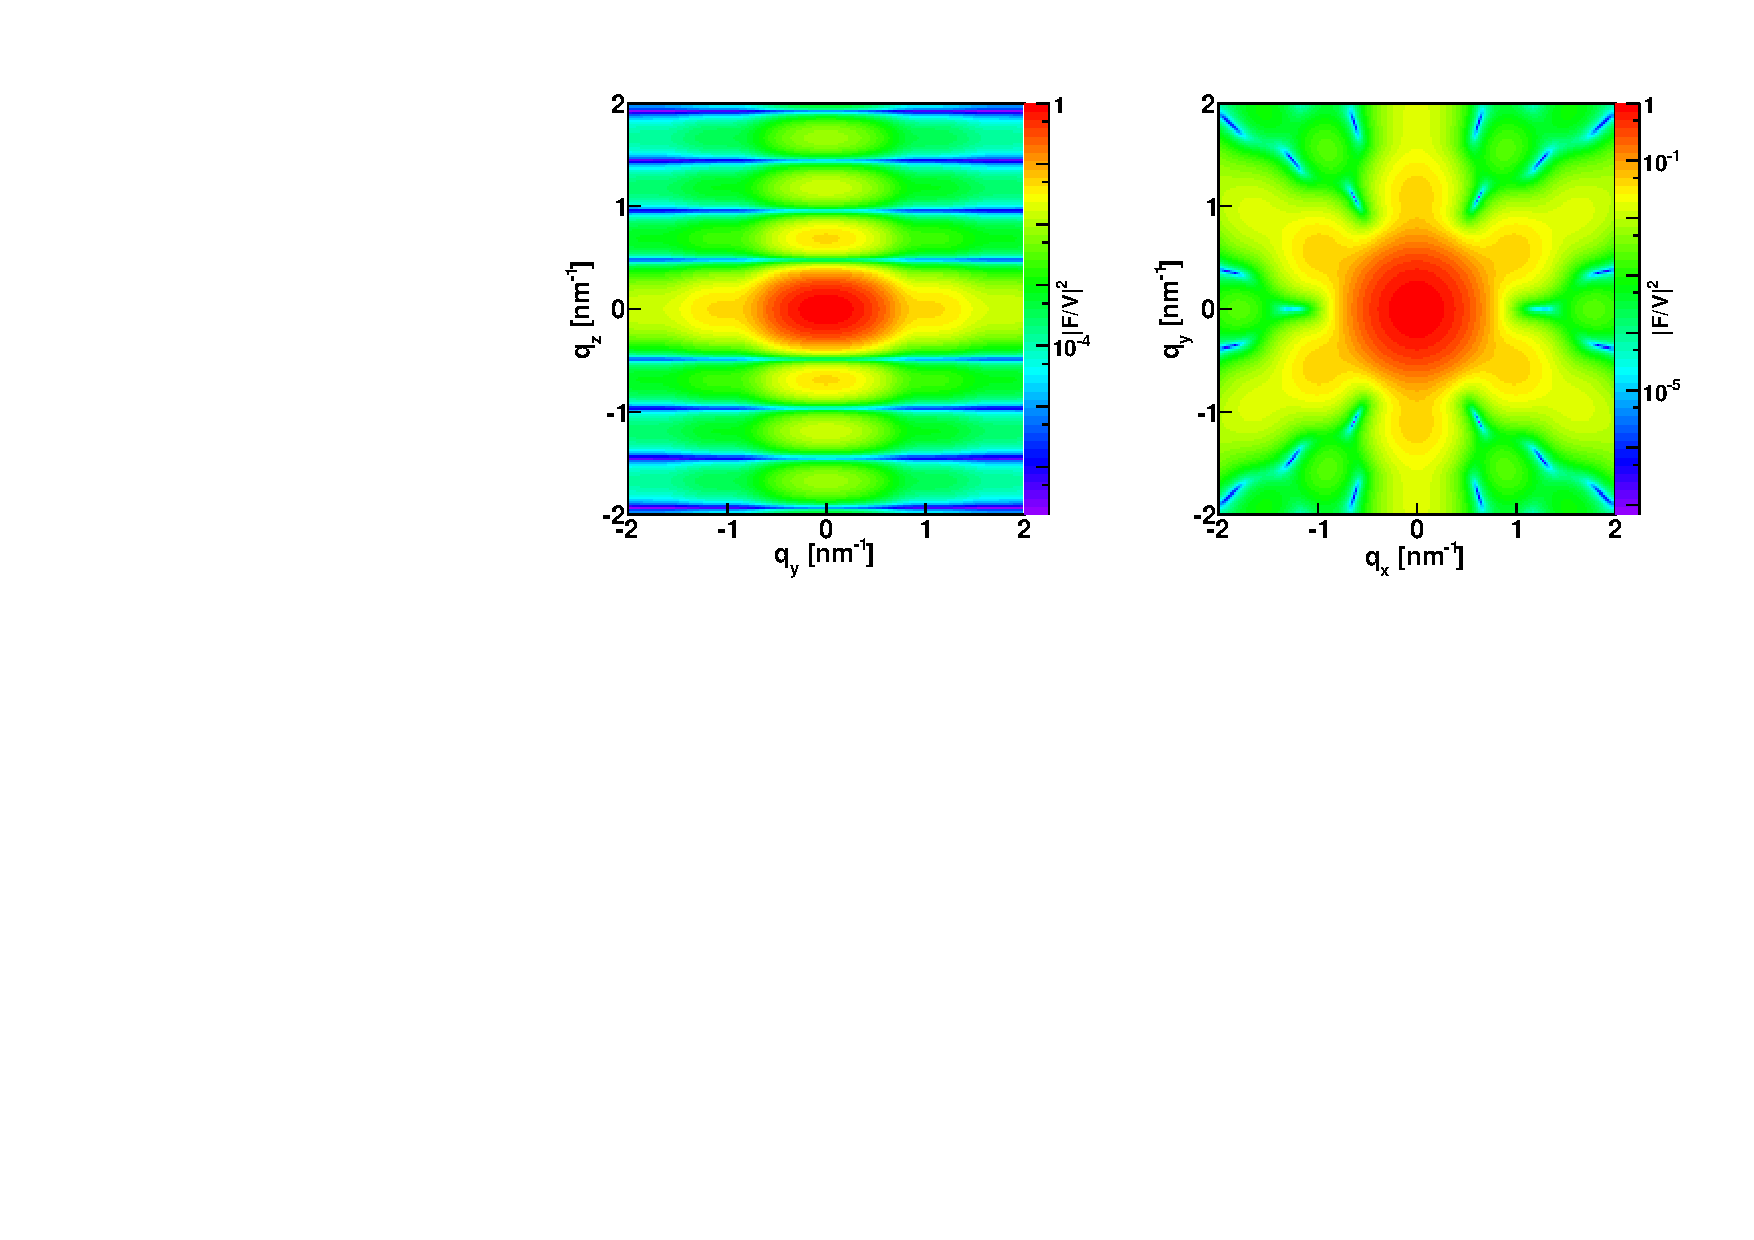
\includegraphics[width=0.9\textwidth]{Figures/figffprism3}
\end{center}
\caption{Normalized intensity for the form factor of a Prism3
  $|F|^2/V^2$, plotted against ($q_z$, $q_y$) and  ($q_x$, $q_y$) and
  computed with $L=10$~nm and $H=13$~nm.}
\label{figFFprism3Ex}
\end{figure}

\subsection{References}
In the $x,y$ plane , we use the full side length of the triangular
base instead of  half as implemented in \Code{IsGISAXS}: $L= 2
R_{\rm{\Code{IsGISAXS}}}$.

\newpage{\cleardoublepage}
%%%%%%%%%%%%%%%%%%%%%%%%%%%%%%%%%%%%
\section{Tetrahedron}  \SecLabel{Tetrahedron} 
 
\subsection{Real-space geometry}
This shape is a truncated tetrahedron as shown in fig.~\ref{tetrahedron}.

\begin{figure}[ht]
\begin{center}
%\includegraphics[width=0.6\columnwidth]{Figures/Tetrahedron}
\caption{Sketch of a tetrahedron.}
\end{center}
\label{tetrahedron}
\end{figure}

\paragraph{Parameters:}
\begin{itemize}
\item length of one side of the equilateral triangular base $L$,
\item height $H$,
\item angle $\alpha$ is the angle between the base and the
  side faces, taken in the middle of the base lines.
\end{itemize}

\paragraph{Restrictions on the parameters:} $\dfrac{H}{L}< \dfrac{\tan{\alpha}}{2\sqrt{3}}$.

\paragraph{Properties:}
\begin{itemize}
\item volume $V= \dfrac{\tan(\alpha)}{24} L^3\Big[1- (1 -
  \sqrt{3}\dfrac{2H}{L \tan(\alpha)} )^3\Big]$,
\item particle surface seen from above $S =\dfrac{\sqrt{3}}{4}L^2$.
%\item radius of gyration
\end{itemize}

\subsection{Expression of the form factor}

\begin{align*}
&F_{\rm{Tetrahedron}} (\mathbf{q}, L, H, \alpha)=\frac{\sqrt{3}H}{q_x (q_x^2-3q_y^2)}
\exp(iq_z \frac{L}{2\tan (\alpha)\sqrt{3}})\\
&\Big\{2q_x \exp(iq_3 D)\sinc(q_3 H) - (q_x +\sqrt{3}q_y)
\exp(iq_1 D)\sinc(q_1 D) -(q_x-\sqrt{3}q_y)\exp(-iq_2
D)\sinc(q_2 H) \Big\} 
\end{align*}
with $\sinc(x)=\sin(x)/x$,
\begin{equation*}
q_1  =\frac{1}{2}\left[\frac{q_x\sqrt{3} -q_y}{\tan \alpha}-q_z \right],
\quad q_2 = \frac{1}{2}\left[\frac{q_x\sqrt{3} +q_y}{\tan \alpha}+q_z
\right], \quad 
q_3 = \frac{q_y}{\tan \alpha} -\frac{q_z}{2}, \quad D = \frac{L \tan \alpha}{\sqrt{3}} -H.
\end{equation*}

\paragraph{Syntax:} \Code{FormFactorTetrahedron(length, height, alpha)}

\subsection{Examples}
Figure~\ref{figFFtetrahEx} shows the normalized intensity
$|F|^2/V^2$, computed with $L=15$~nm, $H=6$~nm and $\alpha =60 ^{\circ}$.
\begin{figure}[h]
\begin{center}
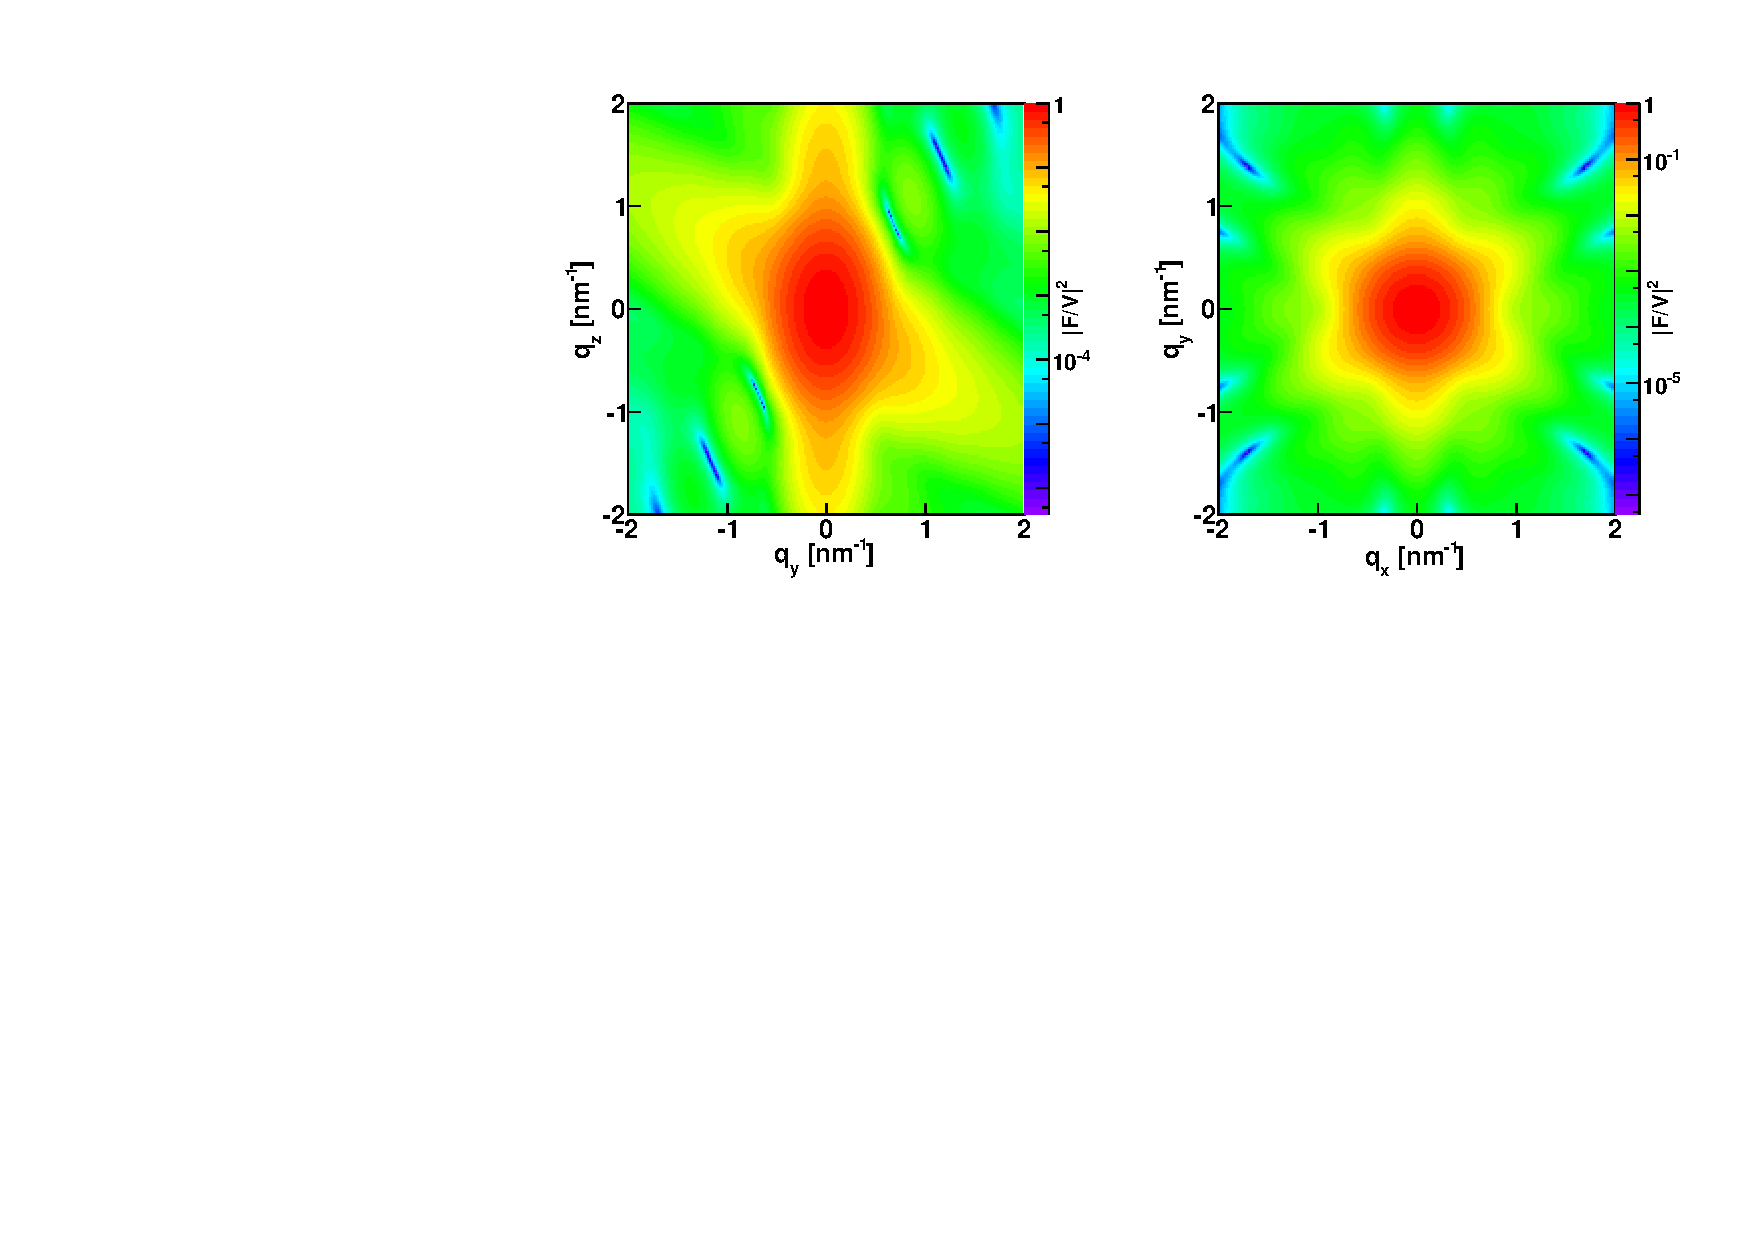
\includegraphics[width=0.9\textwidth]{Figures/figfftetrahedron}
\end{center}
\caption{Normalized intensity for the form factor of a Tetrahedron
  $|F|^2/V^2$, plotted against ($q_z$, $q_y$) and  ($q_x$, $q_y$) and
  computed with $L=15$~nm, $H=6$~nm and $\alpha=60^{\circ}$.}
%Computed results for $R=10$~nm, $H=9$~nm and $\alpha=60^{\circ}$. 
\label{figFFtetrahEx}
\end{figure}

\FloatBarrier

\subsection{References}
%In \Code{IsGISAXS}, factor 1/sqrt(3) instead of sqrt(3) in the
%expression of the form factor. When running the software, there is
%also a problem with this form factor.
In the $x,y$ plane , we use the full side length of the triangular
base instead of  half as implemented in \Code{IsGISAXS}: $L= 2
R_{\rm{\Code{IsGISAXS}}}$.

\newpage{\cleardoublepage}
%%%%%%%%%%%%%%%%%%%%%%%%%%%%%%%%%%%%
\section{Prism6} \SecLabel{Prism6}

\subsection{Real-space geometry}
This shape is an hexagonal prism (see fig.~\ref{prism6}).

\begin{figure}[ht]
\begin{center}
%\includegraphics[width=0.6\columnwidth]{Figures/Prism6}
\caption{Sketch of a Prism6.}
\end{center}
\label{prism6}
\end{figure}


\paragraph{Parameters:}
\begin{itemize}
\item radius of the hexagonal base $R$,
\item height $H$.
\end{itemize}

\paragraph{Properties:}
\begin{itemize}
\item volume $V = \dfrac{3\sqrt{3}}{2}H R^2$,
\item particle surface seen from above $S =\dfrac{3\sqrt{3}R^2}{2}$.
%\item radius of gyration.
\end{itemize}

\subsection{Expression of the form factor}
\begin{align*}
F_{\rm{Prism6}}(\mathbf{q}, R, H) &= \frac{4H\sqrt{3}}{3q_y^2 - q_x^2}
\sinc(\frac{q_z H}{2}) \exp\left(\frac{-i q_z H}{2}\right)\times\\
&\left\{\frac{3q_y^2R^2}{4} \sinc\left(\frac{q_x
  R}{2}\right)\sinc\left(\frac{\sqrt{3}q_yR }{2}\right)+ \cos(q_x R)-\cos\left(q_y
\frac{\sqrt{3}R}{2}\right) \cos\left(\frac{q_x R}{2}\right)\right\}
\end{align*}

\paragraph{Syntax:} \Code{FormFactorPrism6(radius, height)} 

\subsection{Examples}
Figure~\ref{figFFprism6Ex} shows the normalized intensity
$|F|^2/V^2$, computed with $R=5$~nm and $H=13$~nm.

\begin{figure}[h]
\begin{center}
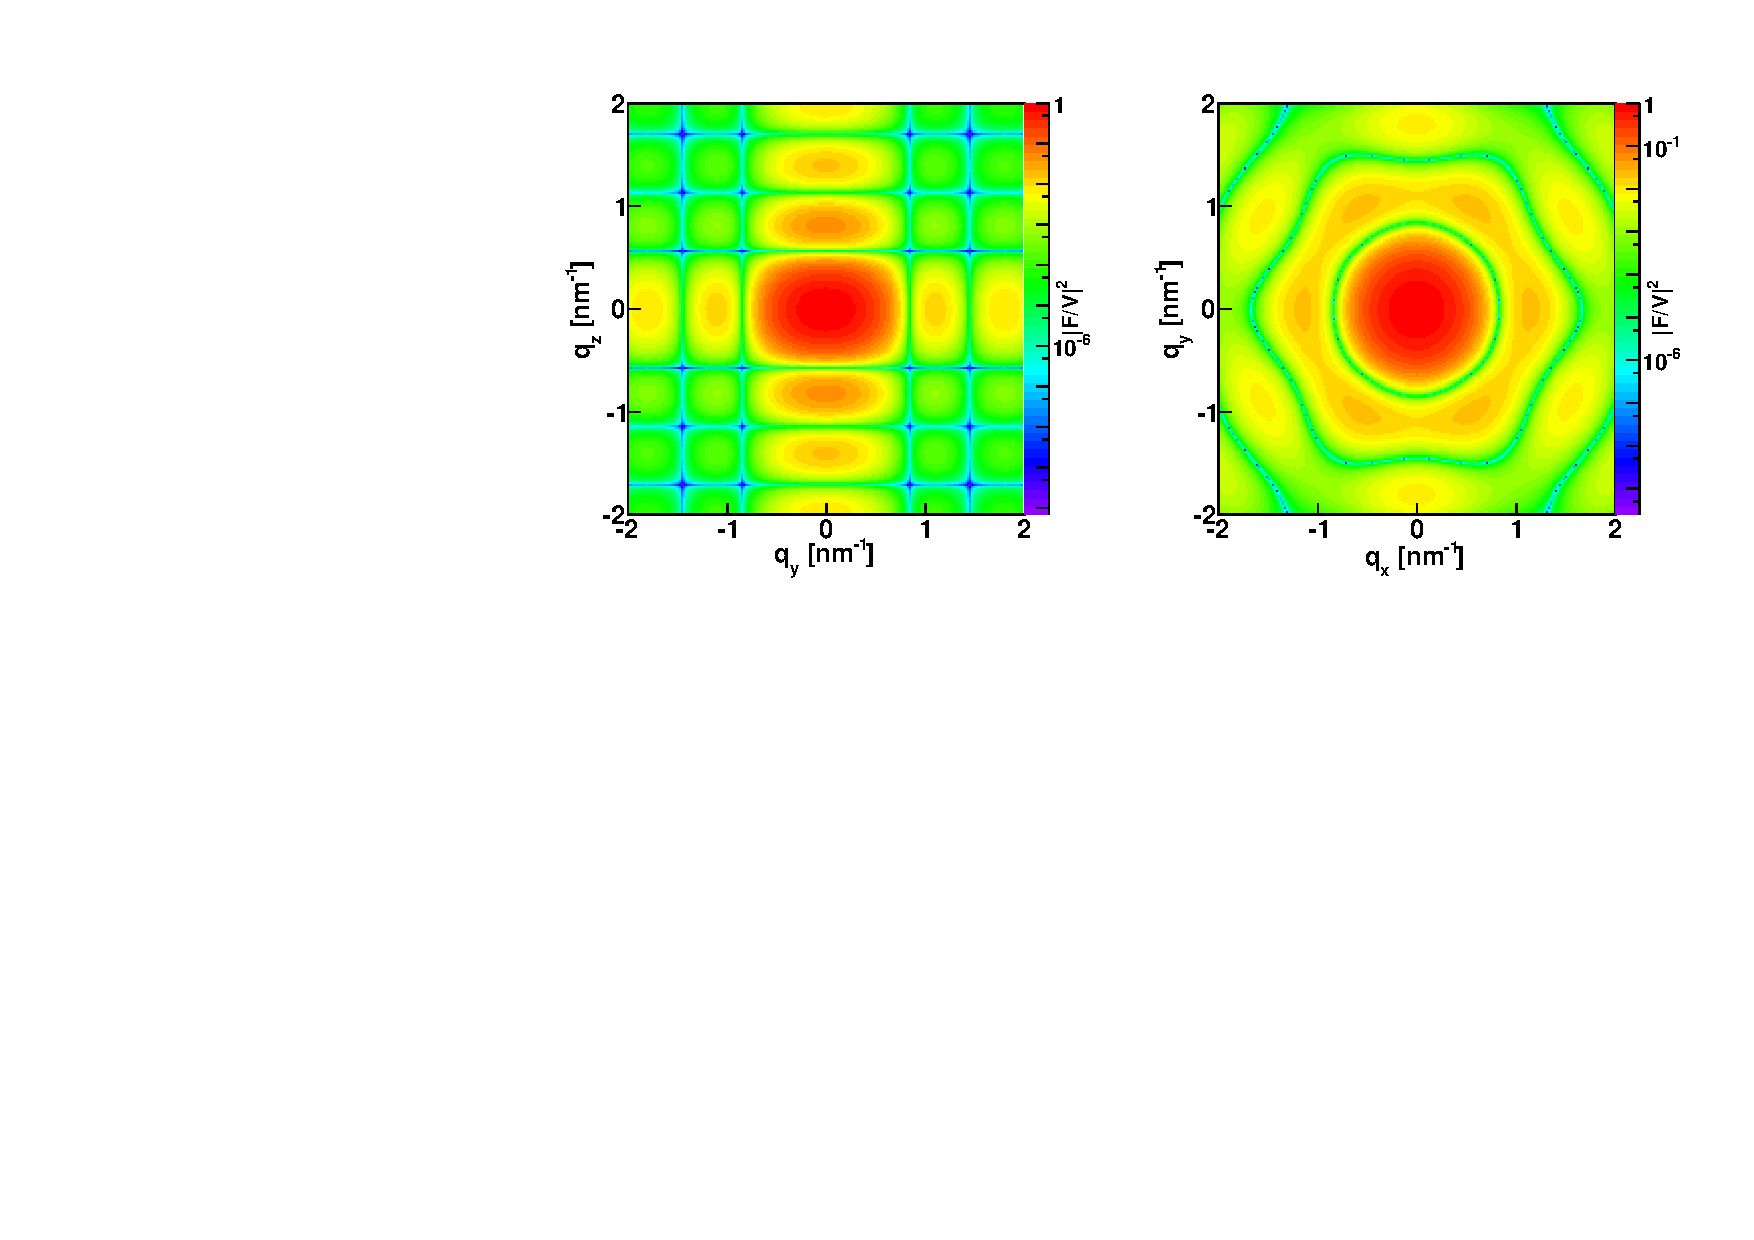
\includegraphics[width=0.9\textwidth]{Figures/figffprism6}
\end{center}
\caption{Normalized intensity for the form factor of a Prism6
  $|F|^2/V^2$, plotted against ($q_z$, $q_y$) and ($q_x$, $q_y$) and computed with $R=5$~nm and $H=13$~nm.}
\label{figFFprism6Ex}
\end{figure}

\FloatBarrier

\subsection{References}
The hexagonal base is parametrized in the different way compared with
\Code{IsGISXAXS}. In \BornAgain\, we use $R = 2/\sqrt{3}R_{\text{\Code{IsGiSaXs}}}$.
%A factor $H$ is missing in the expression of the form factor given in
%\Code{IsGISAXS}'s manual. 


\newpage{\cleardoublepage}
%%%%%%%%%%%%%%%%%%%%%%%%%%%%%%%%%%%%
\section{Cone6} \SecLabel{Cone6} 

\subsection{Real-space geometry}
It is a truncated hexagonal pyramid (see fig.~\ref{cone6}). 

\begin{figure}[ht]
\begin{center}
%\includegraphics[width=0.6\columnwidth]{Figures/Cone6}
\caption{Sketch of a Cone6.}
\end{center}
\label{cone6}
\end{figure}

\paragraph{Parameters:}
\begin{itemize}
\item radius of the regular hexagonal base $R$,
\item height $H$,
\item angle $\alpha$ is considered between one of the side faces and
  the middle of a base length. 
\end{itemize}

\paragraph{Restrictions on the parameters:} $\dfrac{2H}{\sqrt{3}R}< \tan{\alpha}$.

\paragraph{Properties:}
\begin{itemize}
\item volume $V = \dfrac{3}{4} \tan(\alpha) R^3 \Big[
            1 - \big(1- \dfrac{2H}{ \tan(\alpha) R\sqrt{3}}\big)^3
            \Big]$,
\item  particle surface seen from above $S =\dfrac{3\sqrt{3}R^2}{2}$.
%\item radius of gyration
\end{itemize}

\subsection{Expression of the form factor}
The
calculation can be derived from ``Prism6'' (\SecRef{Prism6}) by
considering a side length varying with the vertical position:

\begin{align*}
&F_{\rm{Cone6}}(\mathbf{q}, R, H, \alpha) =\int_0^H
F_{\rm{Prism6}}(R_z)dz\\
&= \frac{4\sqrt{3}}{3q_y ^2 - q_x^2}\int_0 ^H \exp(iq_z z)
\Big[\frac{3}{4}R_z^2q_y^2 \sinc(\frac{q_xR_z}{2})\sinc(\frac{\sqrt{3}}{2}q_y
R_z)+\cos(q_xR_z)-\cos(\frac{\sqrt{3}}{2}q_y R_z)\cos(q_x \frac{R_z}{2}) \Big]dz
\end{align*}
with $R_z=R-\dfrac{2z}{\sqrt{3}\tan(\alpha)}$.

\paragraph{Syntax:} \Code{FormFactorCone6(radius,height, alpha)} 

\subsection{Examples}
Figure~\ref{figFFCone6Ex} shows the normalized intensity
$|F|^2/V^2$, computed with $R=10$~nm, $H=13$~nm, and
$\alpha=60^{\circ}$.

\begin{figure}[h]
\begin{center}
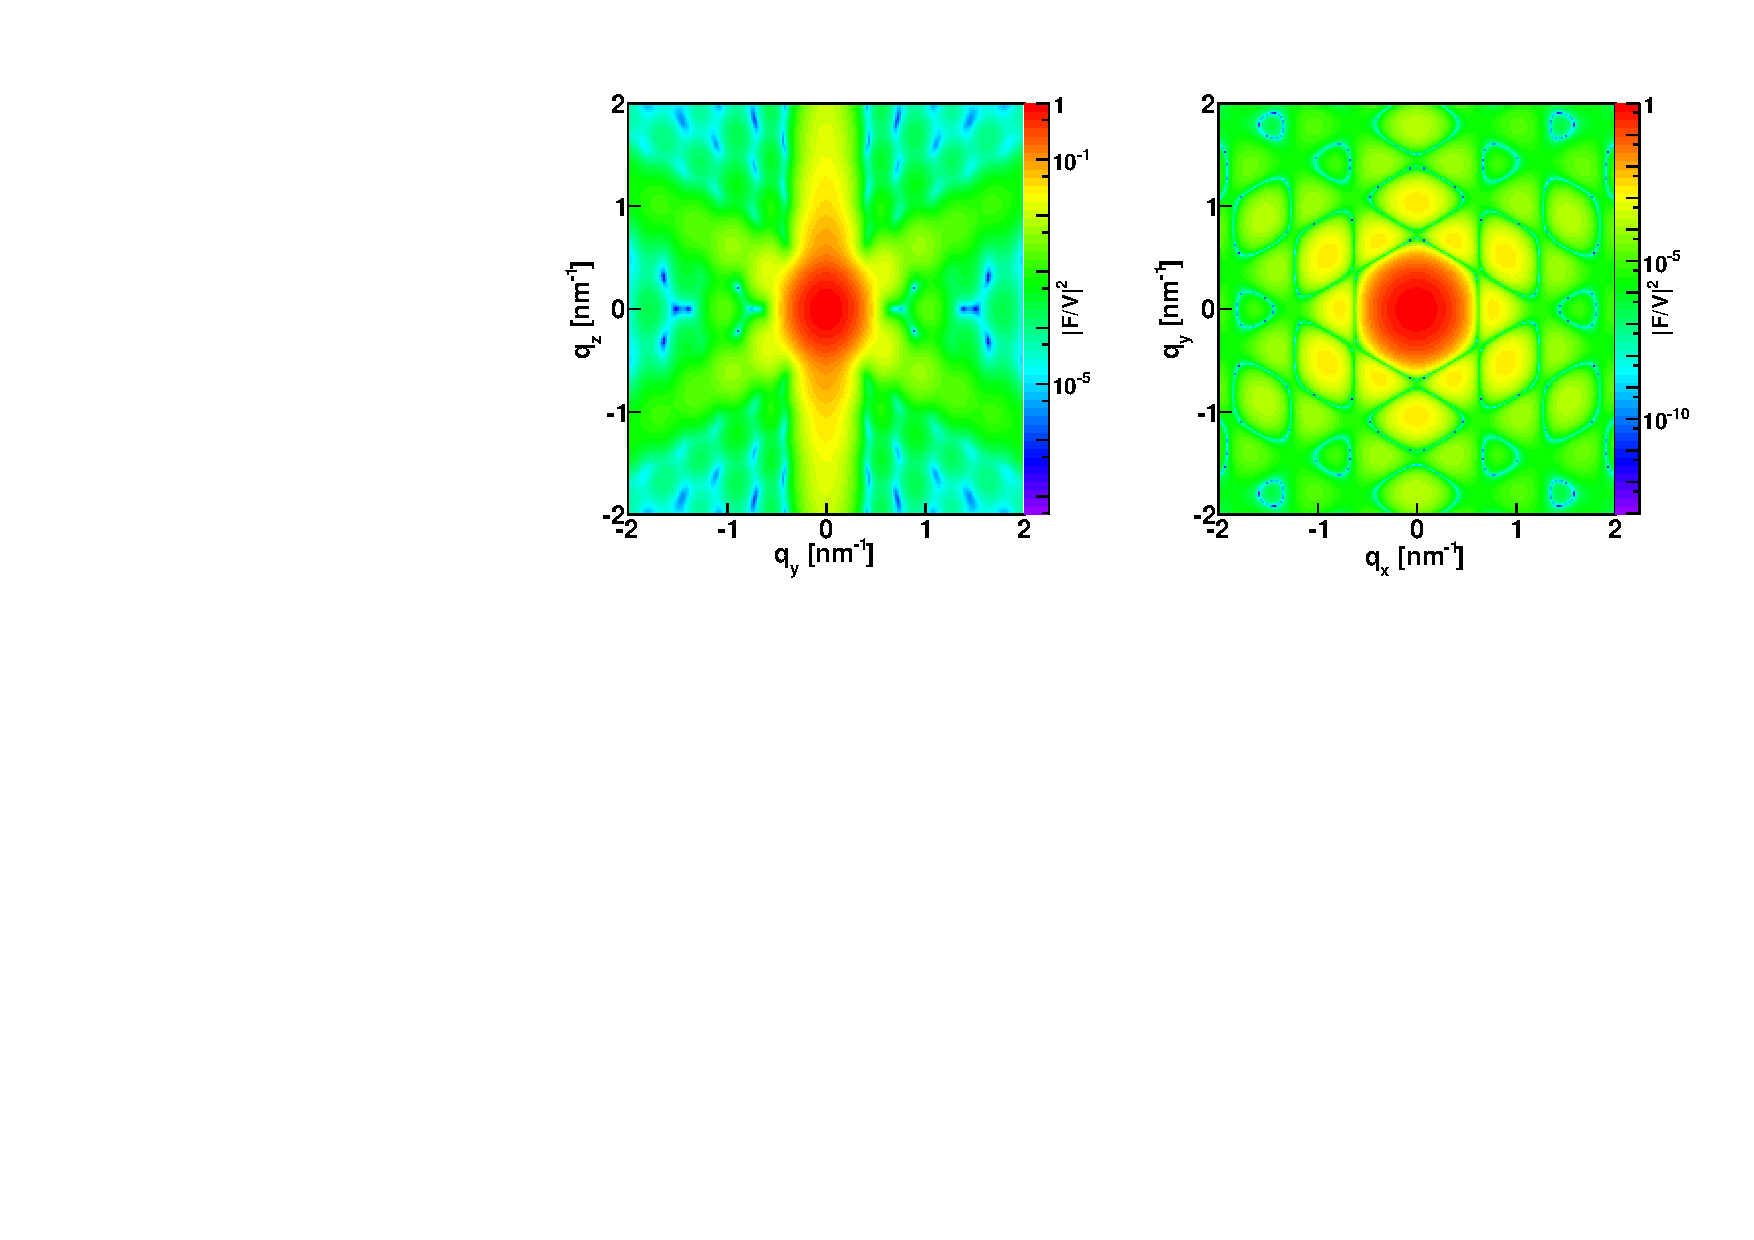
\includegraphics[width=0.9\textwidth]{Figures/figffcone6}
\end{center}
\caption{Normalized intensity for the form factor of a Cone6 $|F|^2/V^2$, plotted against ($q_z$, $q_y$) and ($q_x$, $q_y$) and  computed with $R=10$~nm, $H=13$~nm, and $\alpha=60^{\circ}$.}
\label{figFFCone6Ex}
\end{figure}
\FloatBarrier

\subsection{References}
The convention of the base length is different
from the one implemented in \Code{IsGISAXS}: $R =
2/\sqrt{3}R_{\text{\Code{IsGiSAXS}}}$.

\newpage{\cleardoublepage}
%%%%%%%%%%%%%%%%%%%%%%%%%%%%%%%%%%%%
\section{Pyramid}\SecLabel{Pyramid}

\subsection{Real-space geometry}
This shape is a  truncated pyramid with a square base as shown in fig.~\ref{pyramid}.
\begin{figure}[!h]
\begin{center}
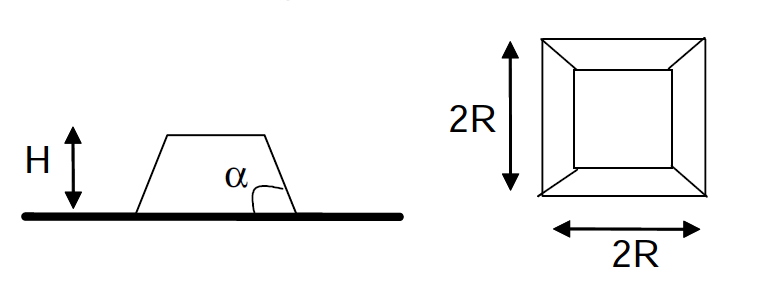
\includegraphics[width=0.6\columnwidth]{Figures/pyramid}
\caption{Sketch of a Pyramid.}
\end{center}
\label{pyramid}
\end{figure} 

\par

\paragraph{Parameters:}
\begin{itemize}
\item length of one side of the square base $L$,  
\item height $H$,
\item  $\alpha$ is the angle between the base and the
  side faces, taken in the middle of the base lines.
\end{itemize}

\paragraph{Restrictions on the parameters:} $\dfrac{2H}{L} < \tan(\alpha)$.

\paragraph{Properties:}
\begin{itemize}
\item  volume $V = \dfrac{1}{6} \tan(\alpha) L^3\Big[ 1
             - \big(1 - \dfrac{2H}{\tan(\alpha)L}\big)^3 \Big],$
\item particle surface seen from above $S = L^2$.
%\item gyration radius along $z$ axis $R_g = \sqrt{2}R$
\end{itemize}

\subsection{Expression of the form factor}
\begin{align}
F_{\rm{Pyramid}}(\mathbf{q},L, H, \alpha) &=
\frac{H}{q_x q_y} \times \nonumber \\ &\Big\{ K_1 \cos[
  (q_x-q_y)L/2 ] + K_2 \sin[ (q_x-q_y)L/2 ]
- K_3 \cos[ (q_x+q_y) L/2 ] - K_4 \sin[ (q_x+q_y) L/2 ]\Big\},
\label{eq:ffpyramid}
\end{align}
with $\sinc(x)=\sin(x)/x$,
\begin{align*}
       q_1 &=\frac{1}{2}\Big[\frac{q_x-q_y}{\tan(\alpha)} + q_z\Big],\quad       q_2 =\frac{1}{2}\Big[\frac{q_x-q_y}{\tan(\alpha)} - q_z\Big]\\
        q_3 &=\frac{1}{2}\Big[\frac{q_x+q_y}{\tan(\alpha)} + q_z\Big],\quad       q_4 =\frac{1}{2}\Big[\frac{q_x+q_y}{\tan(\alpha)} - q_z\Big]\\
        K_1 &= \sinc(q_1 H)\exp(i q_1 H)  + \sinc(q_2 H) \exp(-i q_2 H)\\
        K_2 &= -i \sinc(q_1 H) \exp(i q_1 H) +i \sinc(q_2 H) \exp(-i q_2 H)\\
        K_3 &= \sinc(q_3 H) \exp(i q_3 H)    + \sinc(q_4 H) \exp(-i q_4 H)\\
        K_4 &= -i \sinc(q_3 H) \exp(i q_3 H) + i \sinc(q_4 H) \exp(-i q_4 H) 
   \end{align*}

\paragraph{Syntax:}  \Code{FormFactorPyramid(length, height, alpha)}

\subsection{Examples}
Figure~\ref{figFFPyramidEx} shows the normalized intensity
$|F|^2/V^2$, computed with $L=20$~nm, $H=13$~nm and
$\alpha=60^{\circ}$.

\begin{figure}[h]
\begin{center}
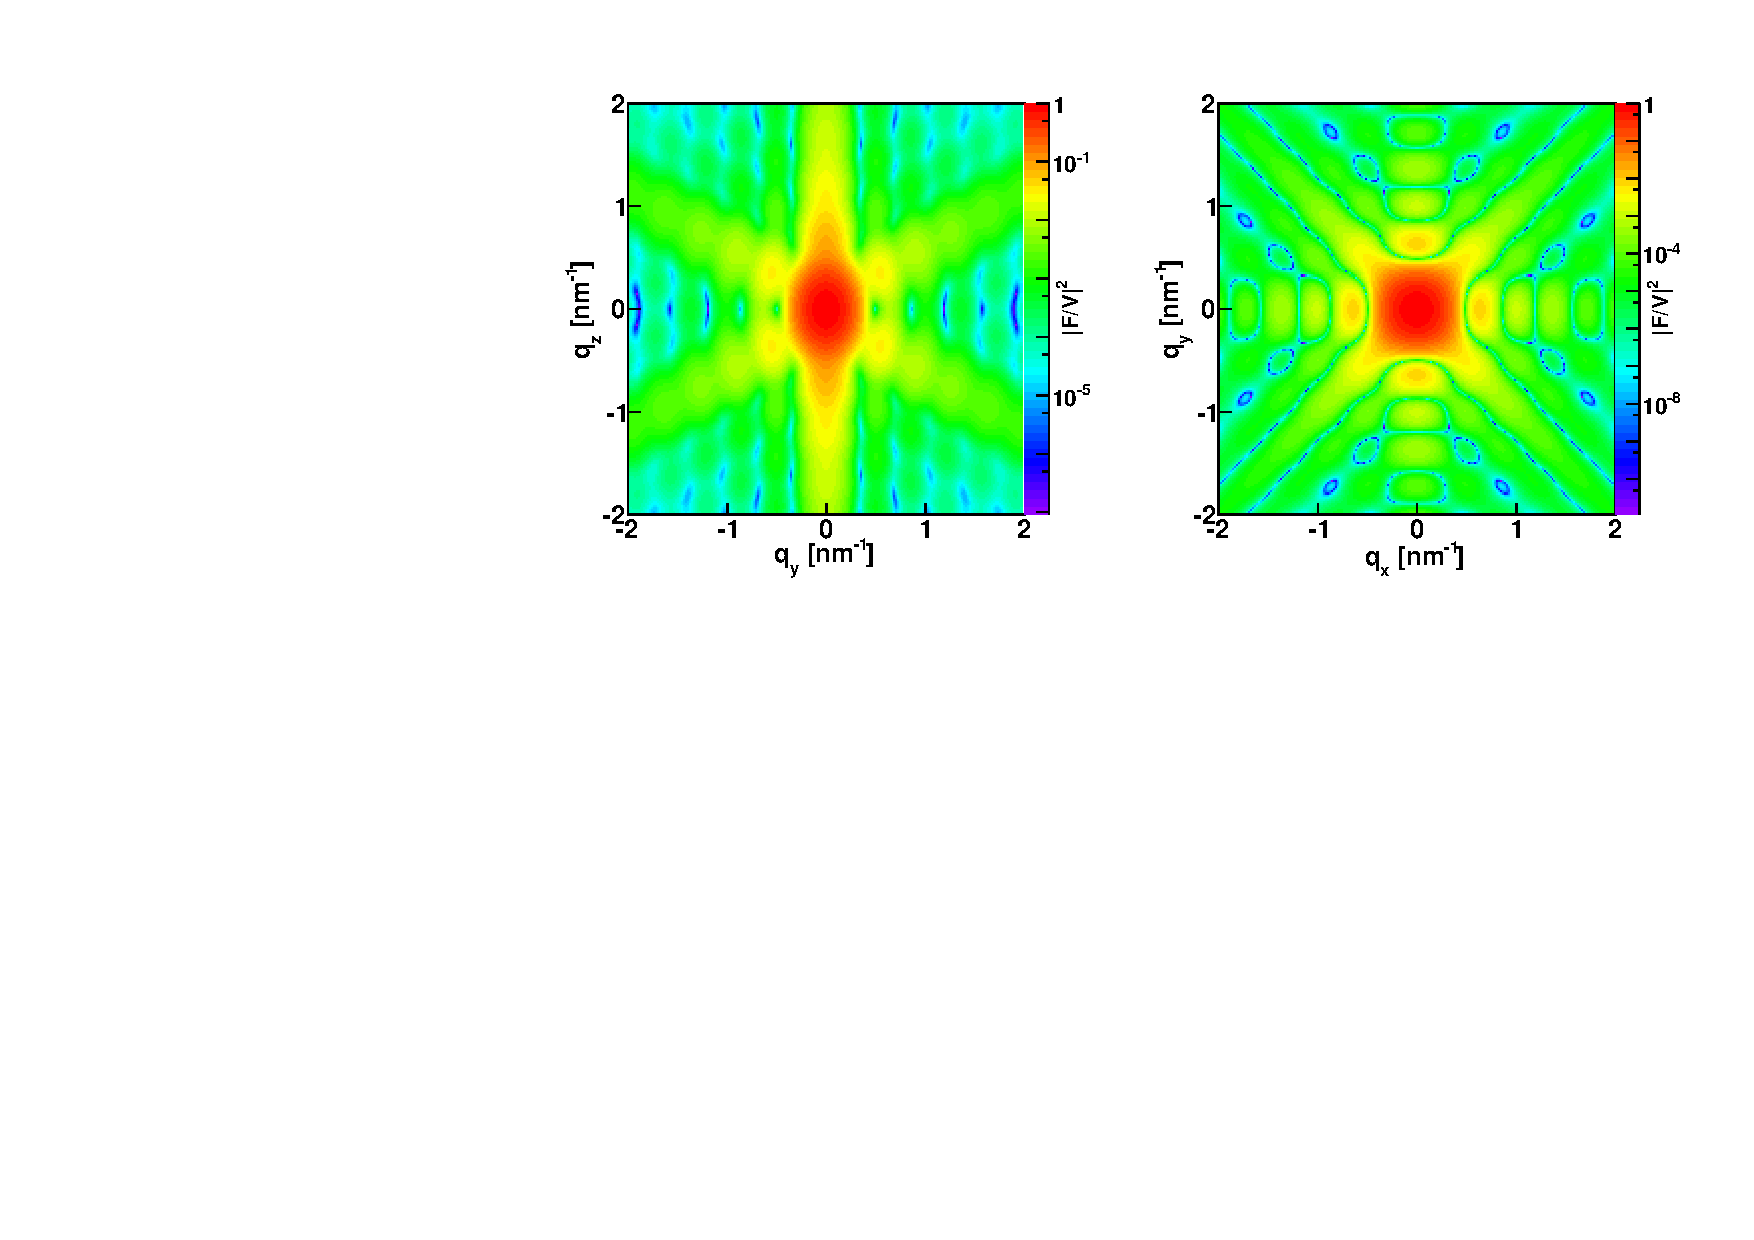
\includegraphics[width=0.9\textwidth]{Figures/figffpyramid}
\end{center}
\caption{Normalized intensity for the form factor of a
  pyramid $|F|^2/V^2$, plotted against ($q_z$, $q_y$) and  
  ($q_x$, $q_y$) and computed with $L=20$~nm and $H=13$~nm, and $\alpha=60^{\circ}$.}
\label{figFFPyramidEx}
\end{figure}

\FloatBarrier

\subsection{References}
The output of equation~(\ref{eq:ffpyramid}) agrees with the \lq\lq
pyramid\rq\rq ~form factor of \IsGISAXS~\cite{Laz02}.

In \BornAgain\, the base of the pyramid is characterized by the full
length of one of its side and not by half this value: $L=2R_{\rm{\Code{IsGISXAXS}}}$. 
%Pyramid: problem with signs of K2 and K4


\newpage{\cleardoublepage}
%%%%%%%%%%%%%%%%%%%%%%%%%%%%%%%%%%%%
\section{Anisotropic pyramid} \SecLabel{AnisoPyramid} 

\subsection{Real-space geometry}
This shape is a truncated right pyramid with a rectangular base as
shown in fig.~\ref{anisopyramid}.

\begin{figure}[ht]
\begin{center}
%\includegraphics[width=0.6\columnwidth]{Figures/Anistropic_pyramid}
\caption{Sketch of an Anisotropic Pyramid. }
\end{center}
\label{anisopyramid}
\end{figure}

\paragraph{Parameters:}
\begin{itemize}
\item full length of the base $L$,
\item full width of the base $W$,
\item height $H$,
\item $\alpha$ is the angle between the base and the
  side faces, taken in the middle of the base lines.
\end{itemize}

\paragraph{Restrictions on the parameters:} $\dfrac{2H}{L}< \tan(\alpha)$ and $\dfrac{2H}{W}< \tan(\alpha)$.

\paragraph{Properties:}
\begin{itemize}
\item volume $V= H \Big[LW - \dfrac{(L + W)H}{\tan(\alpha)}
   + \dfrac{4}{3} \dfrac{H^2}{\tan^2(\alpha)}\Big]$,
\item particle surface seen from above $S = LW$.
%\item radius of gyration
\end{itemize}

\subsection{Expression of the form factor}
\begin{align*}
&F_{\rm{AnisoPyramid}}(\mathbf{q}, L, W, H, \alpha)=
\frac{H}{q_xq_y} \times \\
&\Big\{
K_1\cos\Big(q_x \frac{L}{2} -q_y \frac{W}{2}\Big)+  K_2 \sin \Big (q_x
\frac{L}{2}- q_y \frac{W}{2}\Big) - K_3 \cos \Big (q_x \frac{L}{2} +q_y \frac{W}{2}\Big)-
K_4 \sin \Big (q_x \frac{L}{2} + q_y \frac{W}{2}\Big)
\Big\}
\end{align*}
with $\sinc(x)=\sin(x)/x$,
\begin{align*}
K_1 &= \exp(-i q_2 H) \sinc(q_2 H) + \exp(iq_1 H) \sinc(q_1 H) \\
K_2 &= i \exp(-iq_2 H) \sinc(q_2 H) -i \exp(iq_1 H) \sinc(q_1 H) \\
K_3 &= \exp(-iq_4 H) \sinc(q_4 H) + \exp(iq_3 H) \sinc(q_3 H) \\
K_4 &= i \exp(i q_4 H) \sinc(q_4 H) -i \exp(iq_3 H) \sinc(q_3 H)\\
q_1 &= \frac{1}{2}\left[\frac{q_x -q_y}{\tan \alpha} +q_z \right],\quad q_2 = \frac{1}{2}\left[\frac{q_x -q_y}{\tan \alpha} -q_z \right]\\
q_3 &= \frac{1}{2}\left[\frac{q_x +q_y}{\tan \alpha} +q_z \right] , \quad q_4 = \frac{1}{2}\left[\frac{q_x +q_y}{\tan \alpha} -q_z \right]
\end{align*}

\paragraph{Syntax:} \Code{FormFactorAnisoPyramid(length, width, height, alpha)}

\subsection{Examples}
Figure~\ref{figFFAnisoPyramidEx} shows the normalized intensity
$|F|^2/V^2$, computed with $L=20$~nm, $W=16$~nm, $H=13$~nm, and
$\alpha=60^{\circ}$.

\begin{figure}[h]
\begin{center}
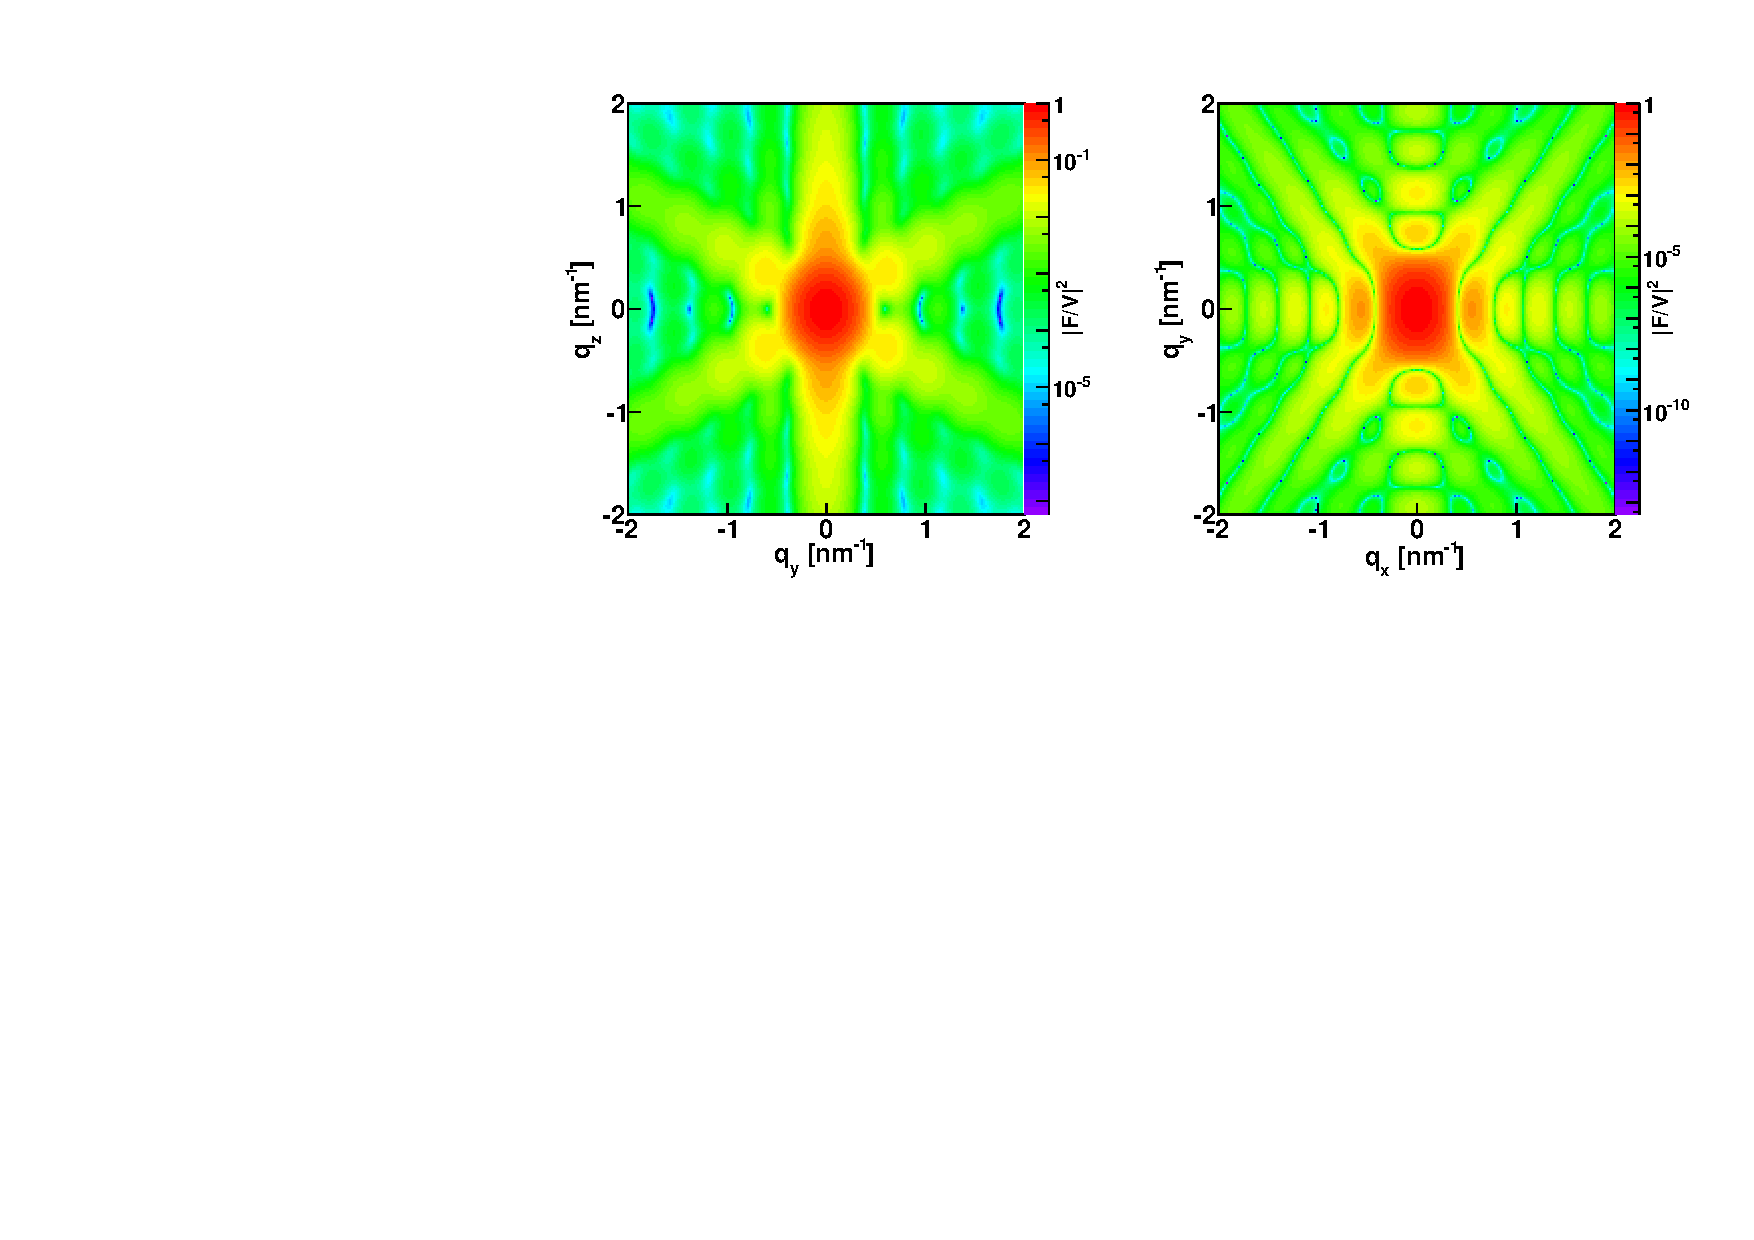
\includegraphics[width=0.9\textwidth]{Figures/figffanisopyramid}
\end{center}
\caption{Normalized intensity for the form factor of an anisotropic
  pyramid $|F|^2/V^2$, plotted against ($q_z$, $q_y$) and  ($q_x$, $q_y$) and computed with $L=20$~nm, $W=16$~nm, $H=13$~nm,
  and $\alpha=60^{\circ}$.}
\label{figFFAnisoPyramidEx}
\end{figure}

\FloatBarrier

\subsection{References}
Like in \Code{IsGISAXS}, the base angle $\alpha$ is the same for both unequal
side. This means that a full anisotropic pyramid is not a limit case. \\
But \BornAgain\ uses a different convention of the parameters relative
to the base. We input the full length and width instead of half values.
%Condition on the parameters: 
%Should not it be: H/R < tan(alpha) and  H/W < tan(alpha) instead of H/R < tan(alpha) and  W/R < tan(alpha) where H is the height and R, W the side-lengths of the rectangular base?

\newpage{\cleardoublepage}
%%%%%%%%%%%%%%%%%%%%%%%%%%%%%%%%%%%%
\section{Cuboctahedron} \SecLabel{Cuboctahedron} 

\subsection{Real-space geometry}
It is a combination of two pyramids with squared bases, as shown in fig.~\ref{cuboctahedron}: the bottom one
is upside down with an height $H$ and the top one has the opposite
orientation (the standard one) and an height $r_H H$.

\begin{figure}[ht]
\begin{center}
%\includegraphics[width=0.6\columnwidth]{Figures/Cubooctaedron}
\caption{Sketch of a Cuboctahedron.}
\end{center}
\label{cuboctahedron}
\end{figure}

\paragraph{Parameters:}
\begin{itemize}
\item length of the shared squared base $L$,
\item height $H$,
\item height\_ratio $r_H$,
\item $\alpha$ is the angle between the base and the
  side faces, taken in the middle of the base lines.
\end{itemize}

\paragraph{Restrictions on the parameters:} $\dfrac{2H}{L}< \tan(\alpha)$ and $\dfrac{2r_HH}{L}< \tan(\alpha)$.

\paragraph{Properties:}
\begin{itemize}
\item volume $ V= \dfrac{1}{6} \tan(\alpha)L^3 \Big[ 2
         - \Big(1 - \dfrac{2H }{L\tan(\alpha)} \Big)^3
           - \Big(1 - \dfrac{2 r_H
             H}{L\tan(\alpha) }\Big)^3\Big]$,
\item particle surface seen from above $S =L^2$.
%\item radius of gyration
\end{itemize}

\subsection{Expression of the form factor}
\begin{equation*}
F_{\rm{Cuboctahedron}}(\mathbf{q}, L, H, r_H, \alpha)=\exp(iq_z
H)\Big[F_{\rm{Pyramid}}(q_x,q_y, q_z, L, r_H H,
\alpha)+F_{\rm{Pyramid}}(q_x, q_y, -q_z, L, H, \alpha))\Big]
\end{equation*}

\paragraph{Syntax:} \Code{FormFactorCuboctahedron(length, height, height\_ratio,
  alpha)}

\subsection{Examples}
Figure~\ref{figFFcuboctahEx} shows the normalized intensity $|F|^2/V^2$, computed with $L=20$~nm, $H=13$~nm, $r_H=0.7$, and $\alpha=60^{\circ}$.
\begin{figure}[h]
\begin{center}
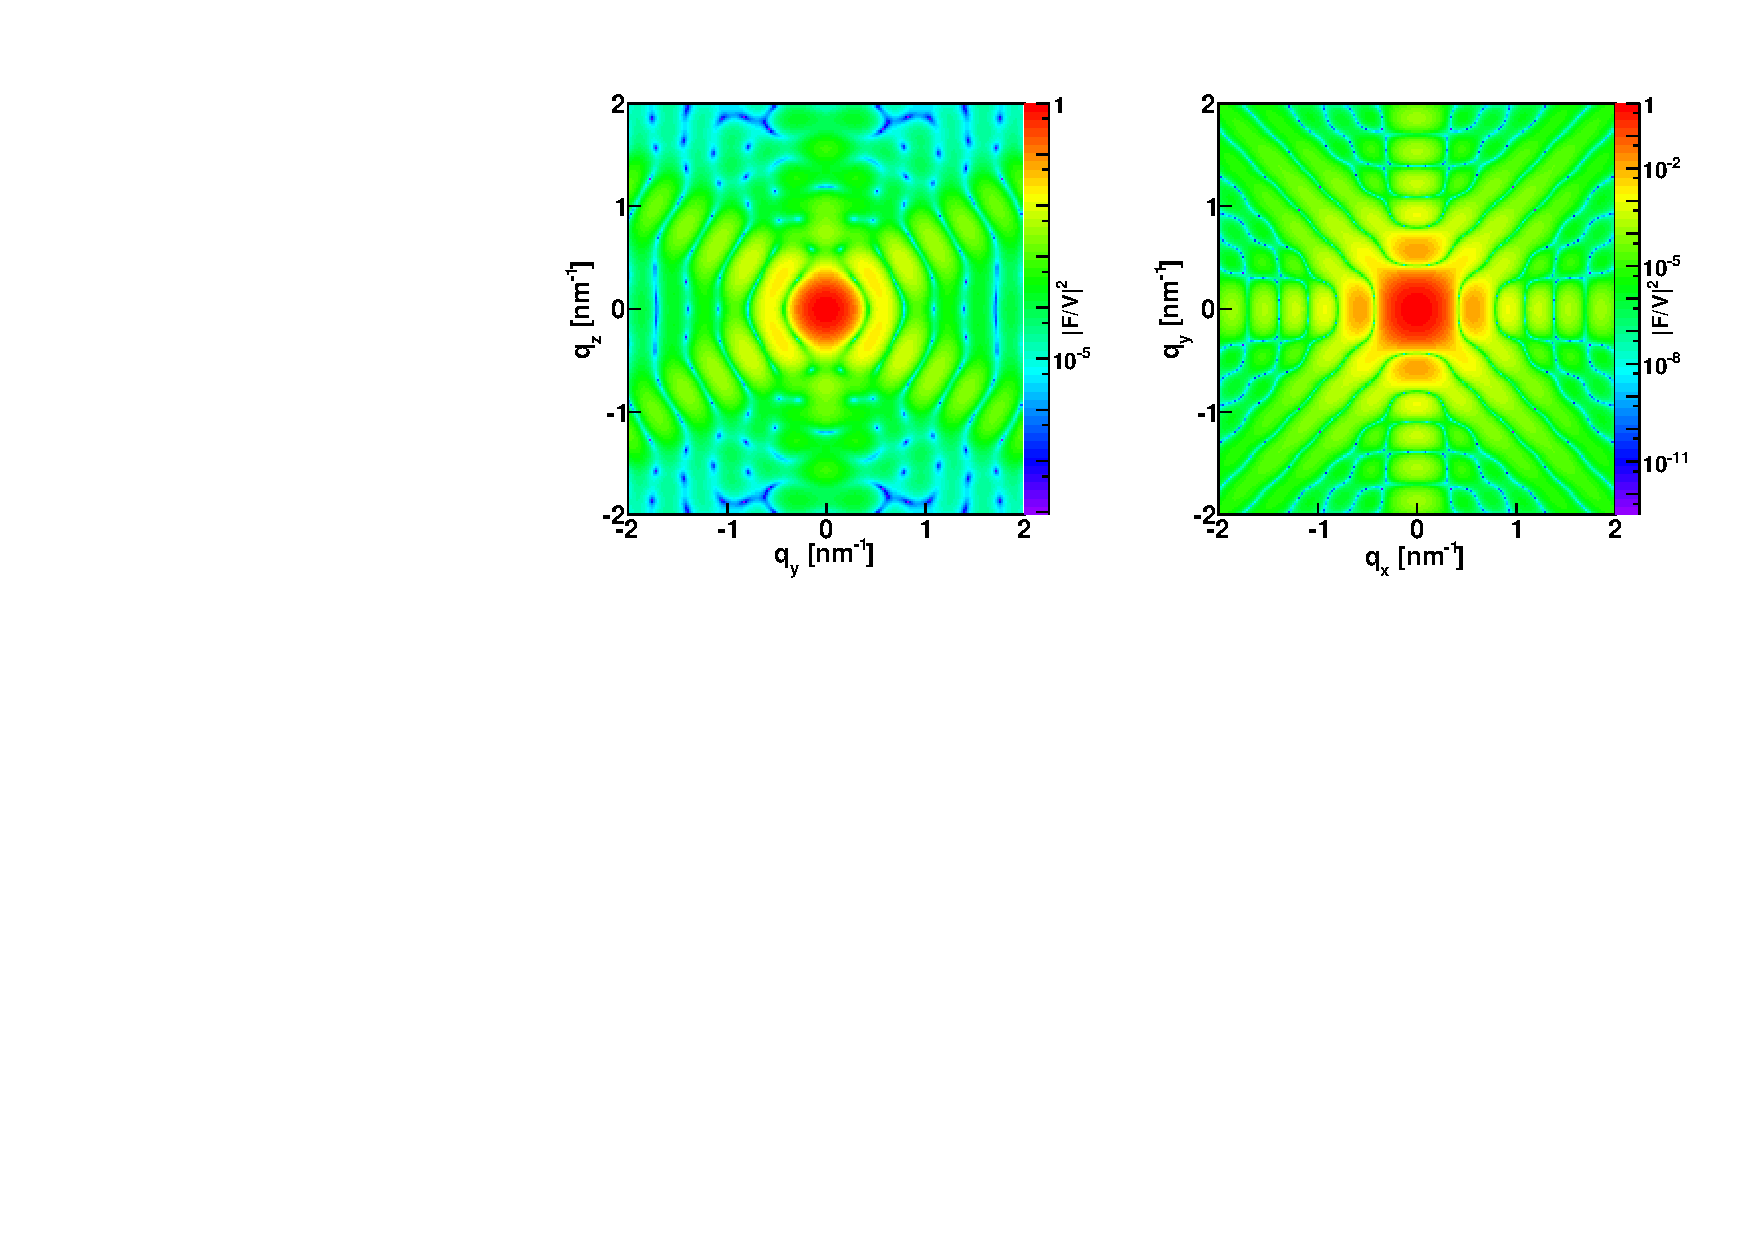
\includegraphics[width=0.9\textwidth]{Figures/figffcuboctah}
\end{center}
\caption{Normalized intensity for the form factor of a cuboctahedron $|F|^2/V^2$, plotted against ($q_z$, $q_y$) and  ($q_x$, $q_y$) and computed with $L=20$~nm, $H=13$~nm,
  $r_H=0.7$, and $\alpha=60^{\circ}$.}
\label{figFFcuboctahEx}
\end{figure}

\FloatBarrier

\subsection{References}
In comparison with \Code{IsGISAXS}, as for the  form factor of a  Pyramid,
we use the full length of a side of the squared base: $L=2R_{\rm{\Code{IsGISAXS}}}$. 
\newpage{\cleardoublepage}
%%%%%%%%%%%%%%%%%%%%%%%%%%%%%%%%%%%%	
\section{Cylinder} \SecLabel{Cylinder}
 
\subsection{Real-space geometry}
This shape is a right circular cylinder (see fig.~\ref{cylinder}).

\begin{figure}[ht]
\begin{center}
%\includegraphics[width=0.6\columnwidth]{Figures/Cylinder}
\caption{Sketch of a Cylinder.}
\end{center}
\label{cylinder}
\end{figure}

\paragraph{Parameters:}
\begin{itemize}
\item radius of the circular base $R$. 
\item height $H$.
\end{itemize}

\paragraph{Properties:}
\begin{itemize}
\item volume $V = \pi R^2 H$,
\item particle surface seen from above $S=\pi R^2$.
%\item radius of gyration
\end{itemize}

\subsection{Expression of the form factor}
  \begin{equation}
F_{\rm{Cylinder}}(\mathbf{q},R, H)=  2\pi
 R^2 H  \sinc(q_ z \frac{H}{2}) \exp(i q_ z \frac{H}{2}) \frac{J_1(q_{\parallel} R )}{q_{\parallel} R }
 \end{equation}
with $q_{\parallel}=\sqrt{q_x^2+q_y^2}$ and $J_1(x)$ is the first order
Bessel function of the first kind \cite{AbSt64}.

\paragraph{Syntax:} \Code{FormFactorCylinder(radius, height)}

\subsection{Examples}
Figure~\ref{figFFcylinderEx} shows the normalized intensity
$|F|^2/V^2$, computed with $R=8$~nm and $H=16$~nm.
\begin{figure}[h]
\begin{center}
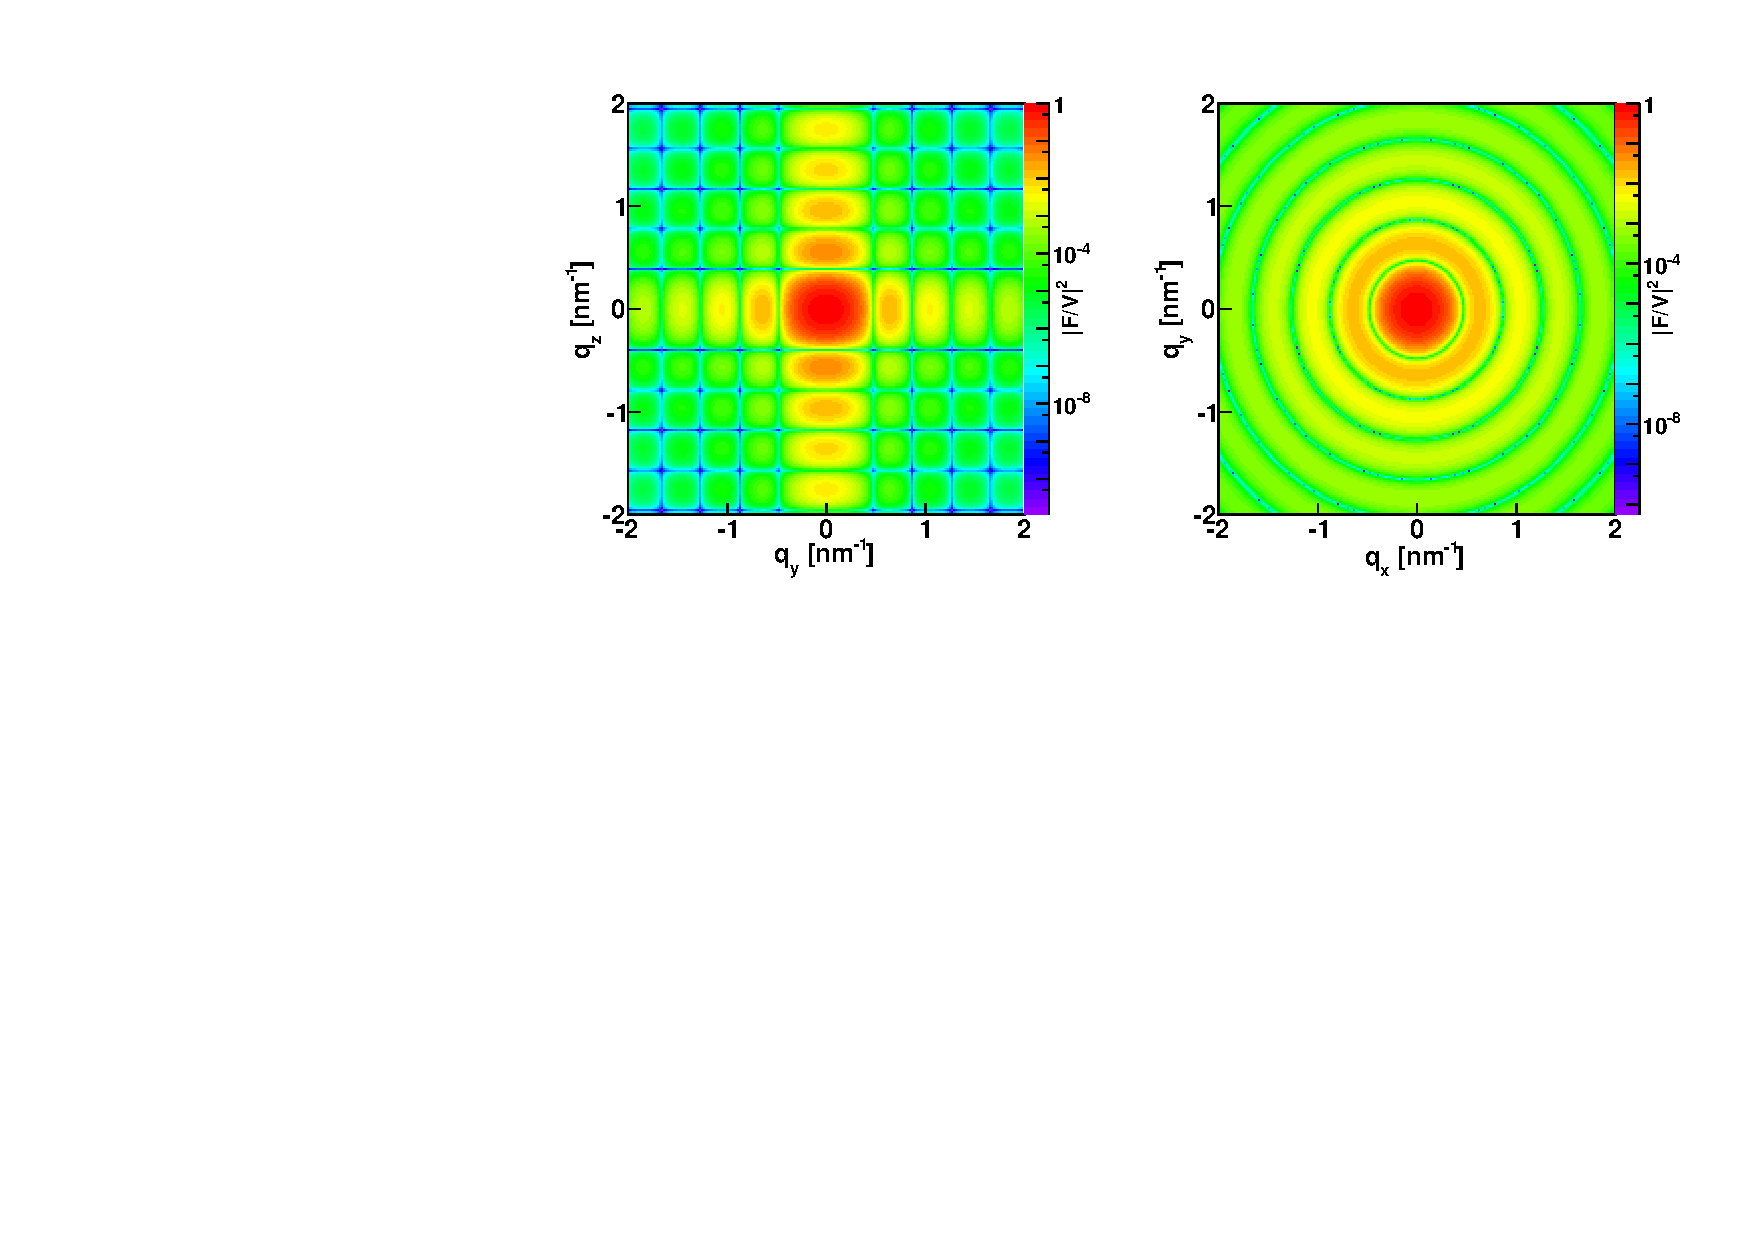
\includegraphics[width=0.9\textwidth]{Figures/figffcylinder}
\end{center}
\caption{Normalized intensity for the form factor of a cylinder
$|F|^2/V^2$, plotted against ($q_z$, $q_y$) and  ($q_x$, $q_y$.) It
has been  computed with $R=8$~nm and $H=16$~nm.}
\label{figFFcylinderEx}
\end{figure}
\FloatBarrier

\subsection{References}

\newpage{\cleardoublepage}
%%%%%%%%%%%%%%%%%%%%%%%%%%%%%%%%%%%%
\section{Ellipsoidal cylinder} \SecLabel{EllipsoidalCylinder} 

\subsection{Real-space geometry}
This is a cylinder whose cross section is an ellipse.

\begin{figure}[ht]
\begin{center}
%\includegraphics[width=0.6\columnwidth]{Figures/Anisotropic_pyramid2}
\caption{Sketch of an Ellipsoidal Cylinder.}
\end{center}
\label{ellipscylinder}
\end{figure}

\paragraph{Parameters:}
\begin{itemize}
\item $r_a$ = half length of the ellipse main axis parallel to $x$,
\item$r_b$ = half length of the ellipse main axis parallel to $y$, 
\item height $H$.
\end{itemize}

\paragraph{Properties:}
\begin{itemize}
\item volume $V = \pi r_a r_bH$,
\item particle surface seen from above $S = r_a r_b$.
%\item radius of gyration
\end{itemize}

\subsection{Expression of the form factor}
The total form factor is given by 
\begin{equation*}
F_{\rm{EllipsoidalCylinder}}(\mathbf{q},R,W,H) = 2\pi r_a r_b H \exp\left(i\frac{q_z
  H}{2}\right)\sinc\left(\frac{q_z H}{2}\right) \frac{J_1(\gamma)}{\gamma},
\end{equation*}
with $\gamma=\sqrt{(q_x r_a)^2+(q_y r_b)^2}$ and $J_1(x)$ is the first order
Bessel function of the first kind \cite{AbSt64}.

\paragraph{Syntax:} \Code{FormFactorEllipsoidalCylinder($r_a$, $r_b$, height)}.

\subsection{Examples}
Figure~\ref{figFFellipscylinderEx} shows the normalized intensity
$|F|^2/V^2$, computed with $r_a=13$~nm, $r_b=8$~nm, and $H=16$~nm.
\begin{figure}[h]
\begin{center}
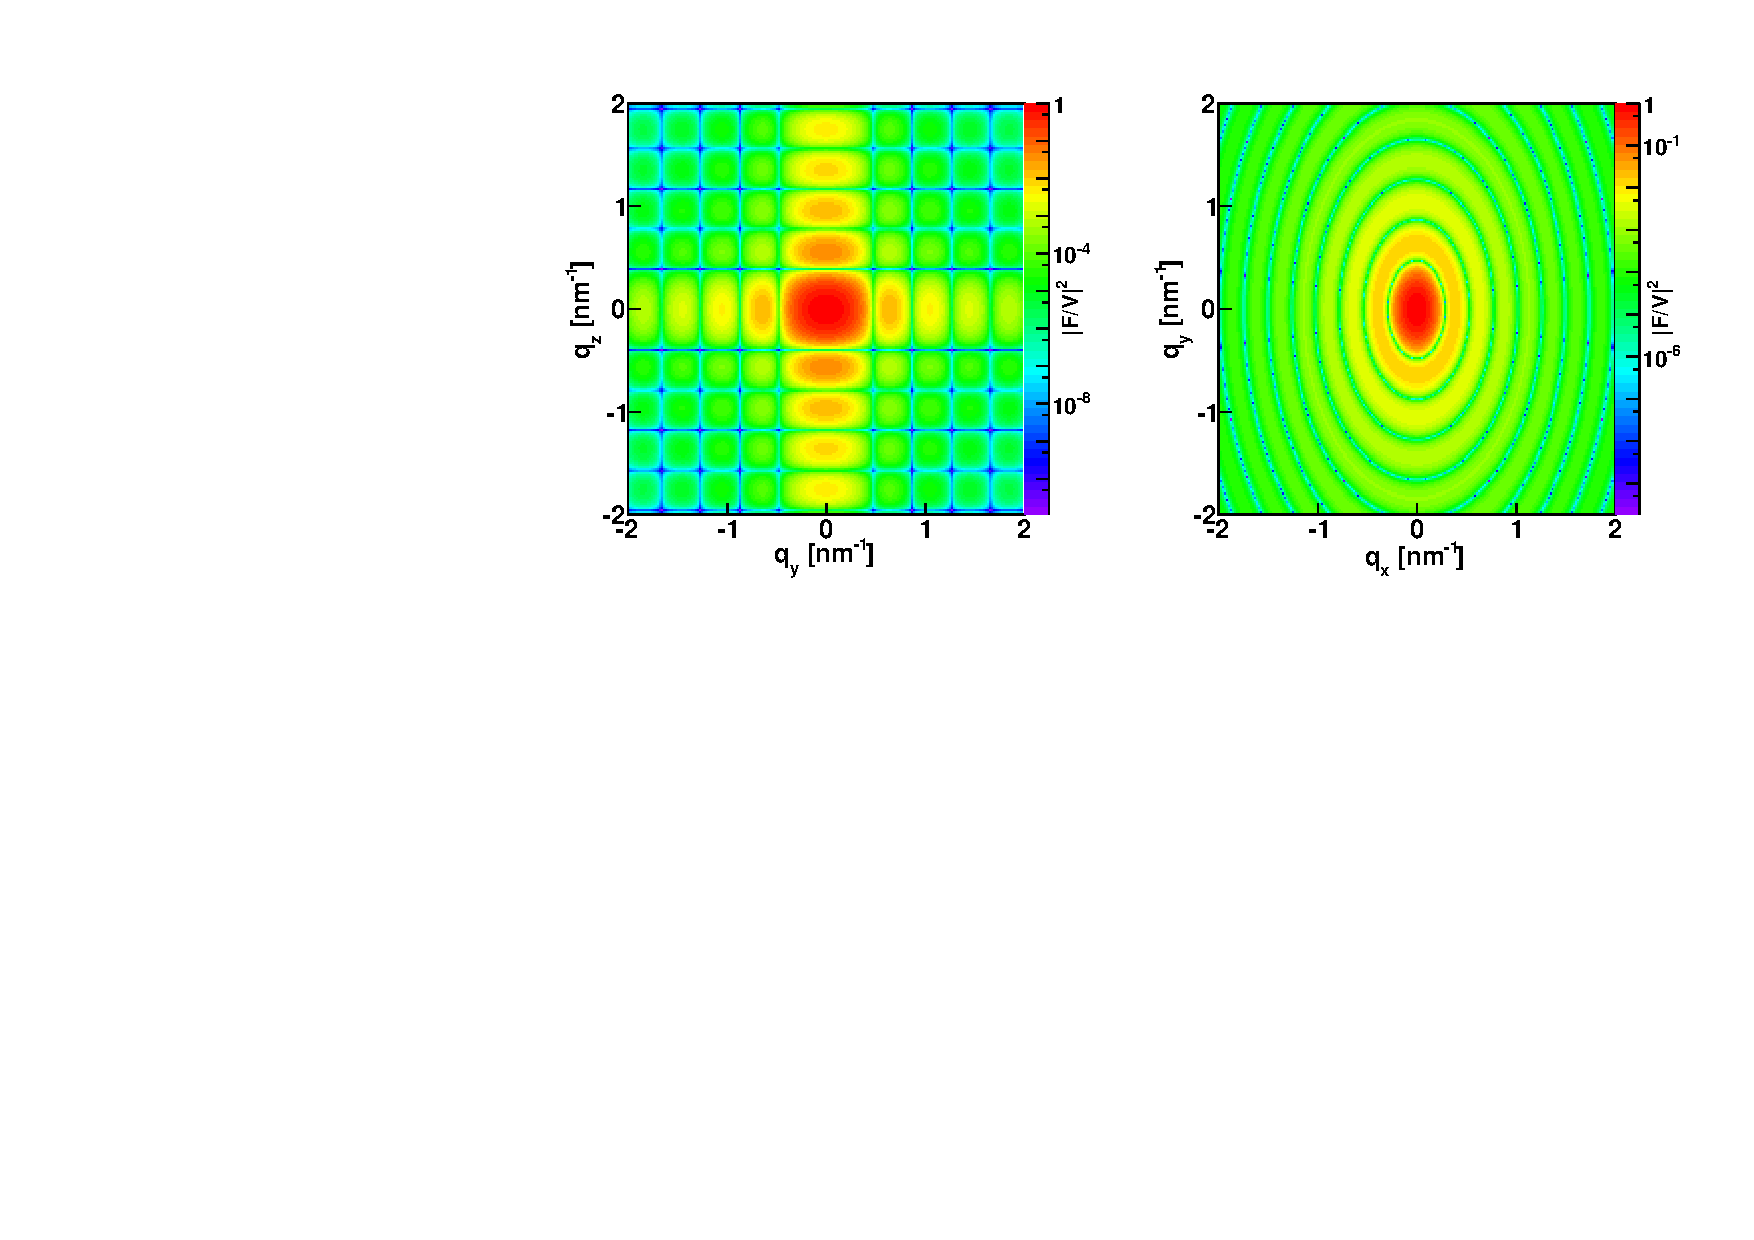
\includegraphics[width=0.9\textwidth]{Figures/figffellipscylinder}
\end{center}
\caption{Normalized intensity for the form factor of an ellipsoidal
  cylinder $|F|^2/V^2$, plotted against ($q_z$, $q_y$) and ($q_x$,
  $q_y$) and computed with $r_a=8$~nm, $r_b=13$~nm, and $H=16$~nm.}
\label{figFFellipscylinderEx}
\end{figure}


\subsection{References}
This form factor is referred to as "Ellipsoid'' in \Code{ISGISAXS}. 

\newpage{\cleardoublepage}
%%%%%%%%%%%%%%%%%%%%%%%%%%%%%%%%%%%%
\section{Cone} \SecLabel{Cone} 

\subsection{Real-space geometry}
This shape is a truncated cone as shown in fig.~\ref{cone}. %Its base is circular with a radius
                                %$R$, its height is equal to $H$. 

\begin{figure}[ht]
\begin{center}
%\includegraphics[width=0.6\columnwidth]{Figures/Cone}
\caption{Sketch of a Cone.}
\end{center}
\label{cone}
\end{figure}

\paragraph{Parameters:}
\begin{itemize}
\item radius $R$,
\item height $H$,
\item $\alpha$ is the angle between the side and the circular base.
\end{itemize}

\paragraph{Restrictions on the parameters:} $\dfrac{H}{R}< \tan(\alpha)$.

\paragraph{Properties:}
\begin{itemize}
\item volume $V = \dfrac{\pi}{3} \tan(\alpha) R^3 \Big[ 
            1 - (1- \dfrac{H}{\tan(\alpha)R})^3\Big]$,
\item  particle surface seen from above $S=\pi R^2$.
%\item radius of gyration
\end{itemize}

\subsection{Expression of the form factor}
\begin{equation*}
F_{\rm{Cone}}(\mathbf{q}, R, H, \alpha) = \int_0 ^H 2\pi R_z^2
\frac{J_1(q_{\parallel}R_z)}{q_{\parallel} R_z}\exp(iq_z z)dz,
\end{equation*}
with $R_z =R-\frac{z}{\tan \alpha}$, $\mathbf{q}_{\parallel}=\sqrt{q_x^2+ q_y^2}$ and $J_1(x)$ is the first order
Bessel function of the first kind \cite{AbSt64}.

\paragraph{Syntax:}  \Code{FormFactorCone(radius, height, alpha)}. 

\subsection{Examples}
Figure~\ref{figFFConeEx} shows the normalized intensity
$|F|^2/V^2$, computed with $R=10$~nm, $H=13$~nm, and $\alpha=60^{\circ}$.
\begin{figure}[h]
\begin{center}
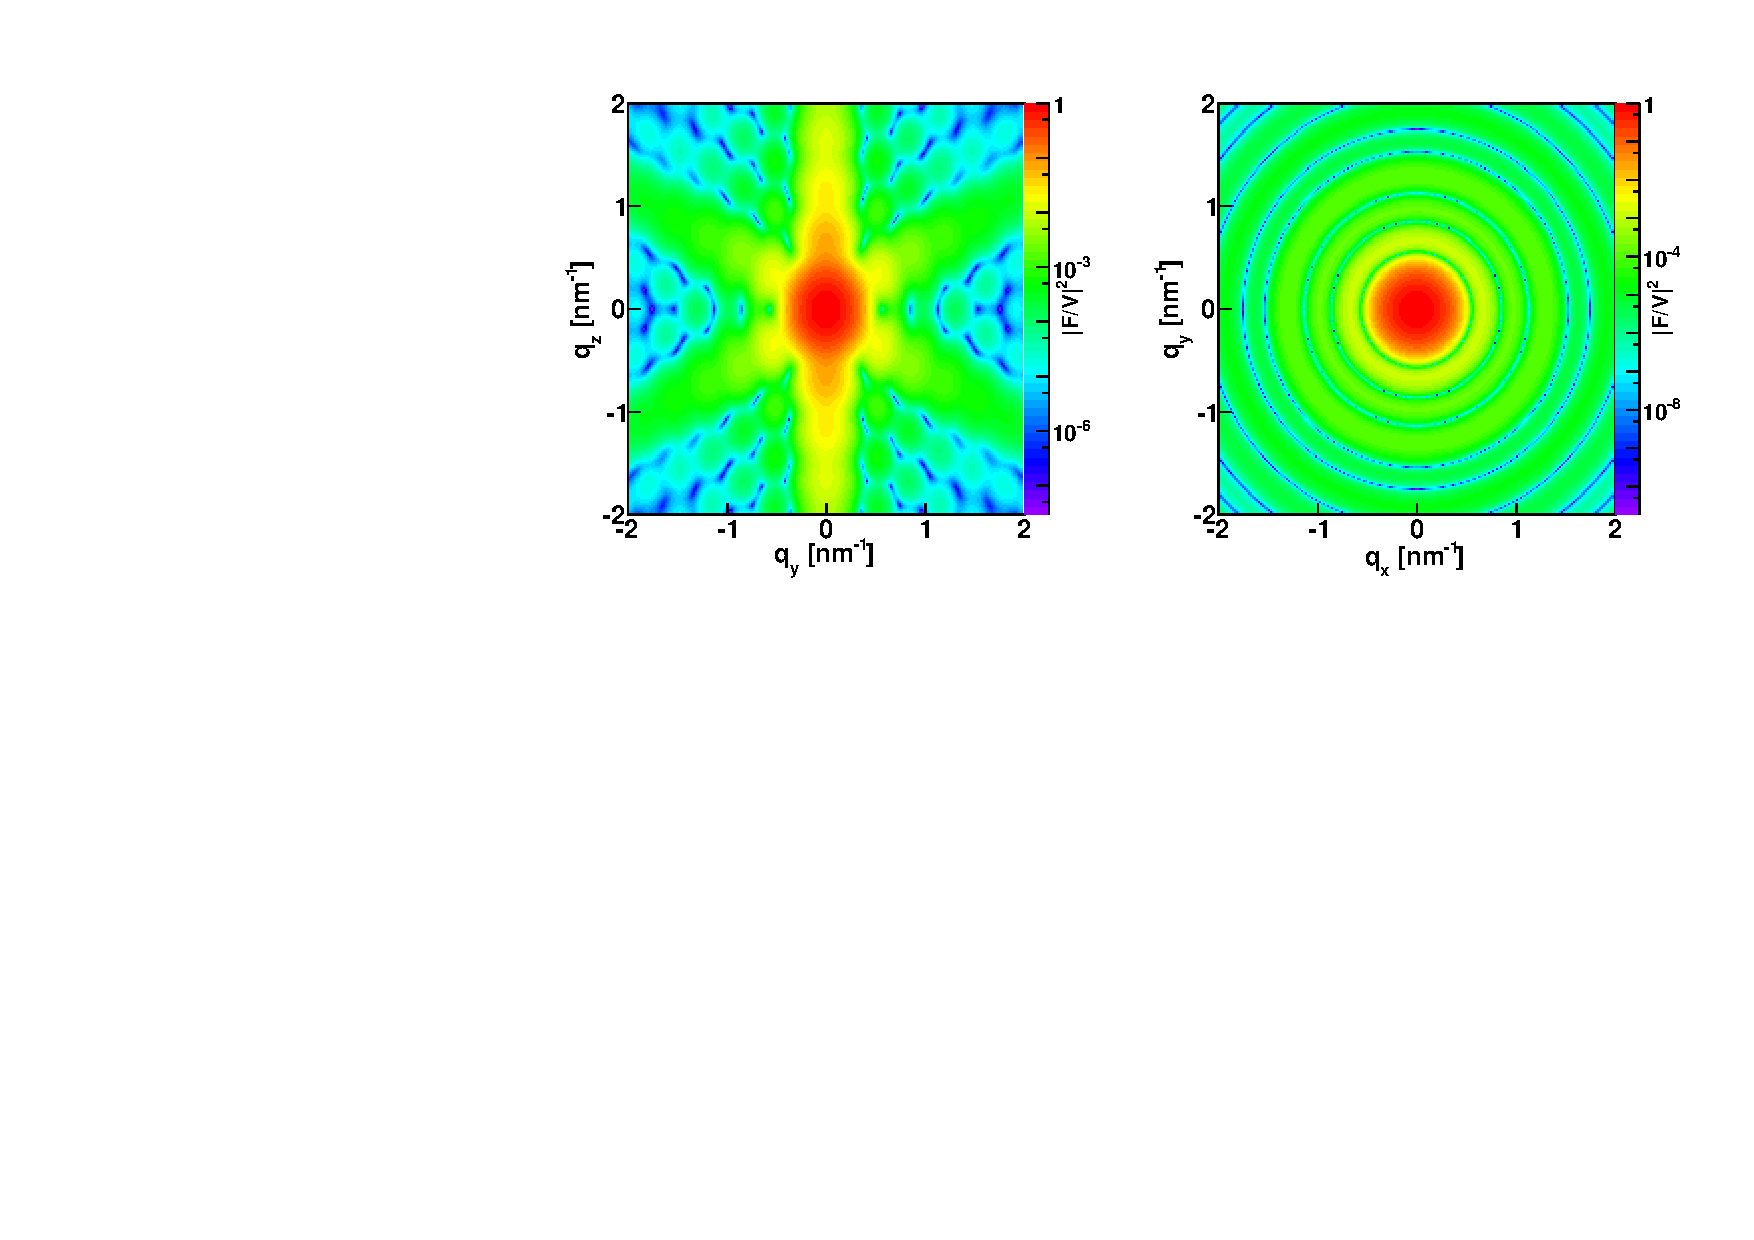
\includegraphics[width=0.9\textwidth]{Figures/figffcone}
\end{center}
\caption{Normalized intensity for the form factor of a Cone
  $|F|^2/V^2$, plotted against ($q_z$, $q_y$) and ($q_x$, $q_y$.) It
  has been  computed with $R=10$~nm, $H=13$~nm,
  and $\alpha=60^{\circ}$.}
\label{figFFConeEx}
\end{figure}


\subsection{References}


\newpage{\cleardoublepage}
%%%%%%%%%%%%%%%%%%%%%%%%%%%%%%%%%%%%
\section{Full sphere} \SecLabel{FullSphere}

\subsection{Real-space geometry}
The full sphere is parametrized by its radius $R$. 
\begin{figure}[ht]
\begin{center}
\includegraphics[width=0.6\columnwidth]{Figures/fullsphere}
\caption{Sketch of a Full Sphere.}
\end{center}
\label{fullsphere}
\end{figure}

\FloatBarrier

\paragraph{Parameters:} radius $R$.

\paragraph{Properties:}
\begin{itemize}
\item volume $V = \dfrac{4\pi}{3}R^3$,
\item particle surface seen from above $S= \pi R^2$.
%\item radius of gyration
\end{itemize}

\subsection{Expression of the form factor}
\begin{equation}
F_{\rm{FullSphere}}(\mathbf{q},R) = 4\pi R^3 \exp(iq_z R)\frac{\sin(q R) - q R \cos(q R)}{(qR)^3},
\end{equation}
where $q=\sqrt{q_x^2 + q_y^2 + q_z^2}$.

\paragraph{Syntax:} \Code{FormFactorFullSphere(radius)}


\subsection{Examples}
Figure~\ref{figFFFSphereEx} shows the normalized intensity $|F|^2/V^2$, computed with $R=8$~nm.
\begin{figure}[h]
\begin{center}
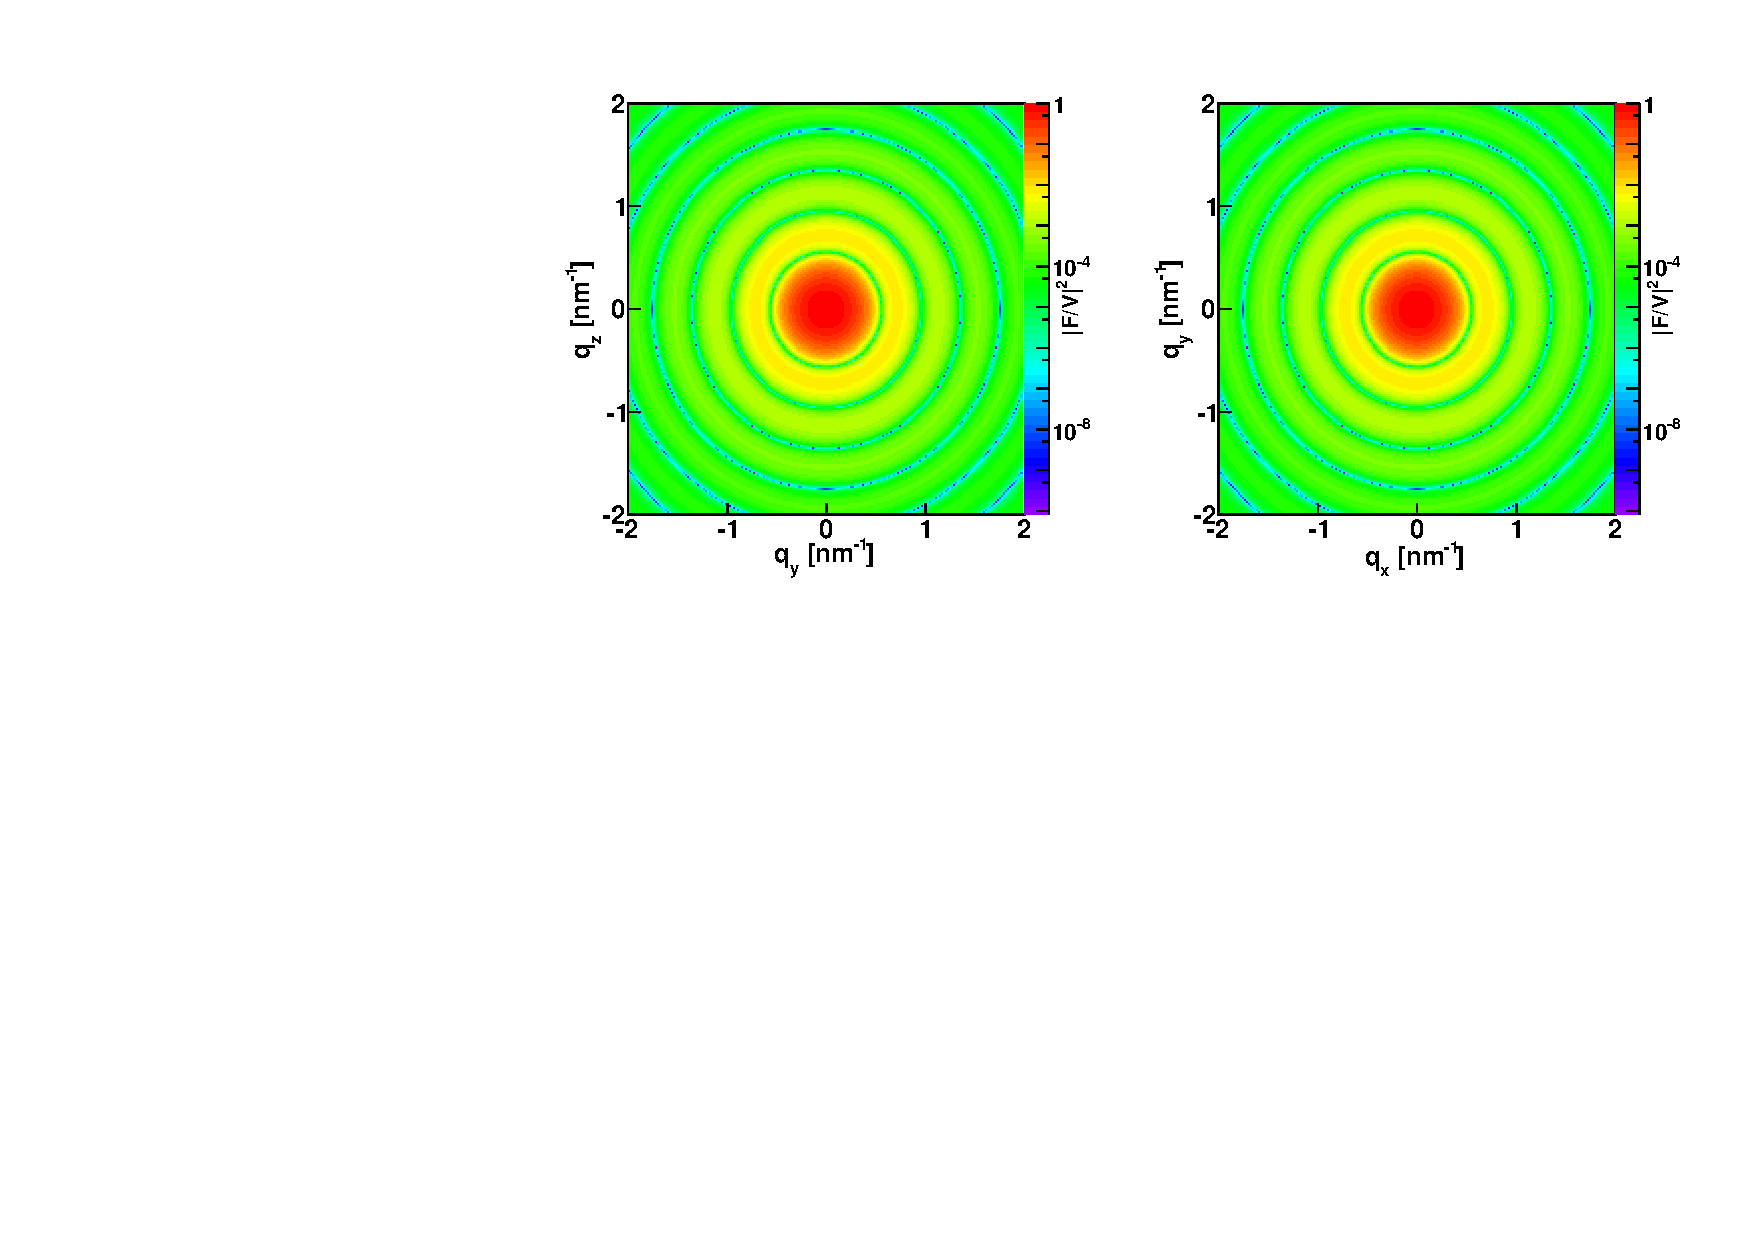
\includegraphics[width=0.9\textwidth]{Figures/figfffsphere}
\end{center}
\caption{Normalized intensity for the
  form factor of a Full Sphere
  $|F|^2/V^2$, plotted against ($q_z$, $q_y$) and ($q_x$, $q_y$) and computed with $R=8$~nm.}
\label{figFFFSphereEx}
\end{figure}

\FloatBarrier

\subsection{References}

%%%%%%%%%%%%%%%%%%%%%%%%%%%%%%%%%%%%
\newpage{\cleardoublepage}
\section{Truncated Sphere}\SecLabel{Sphere}
  
\subsection{Real-space geometry}
This shape is a spherical dome, \textit{i.e.} a portion of a sphere cut off by a plane (perpendicular
to $z$-axis) as shown in fig.~\ref{sphere}.
\begin{figure}[!h]
\begin{center}
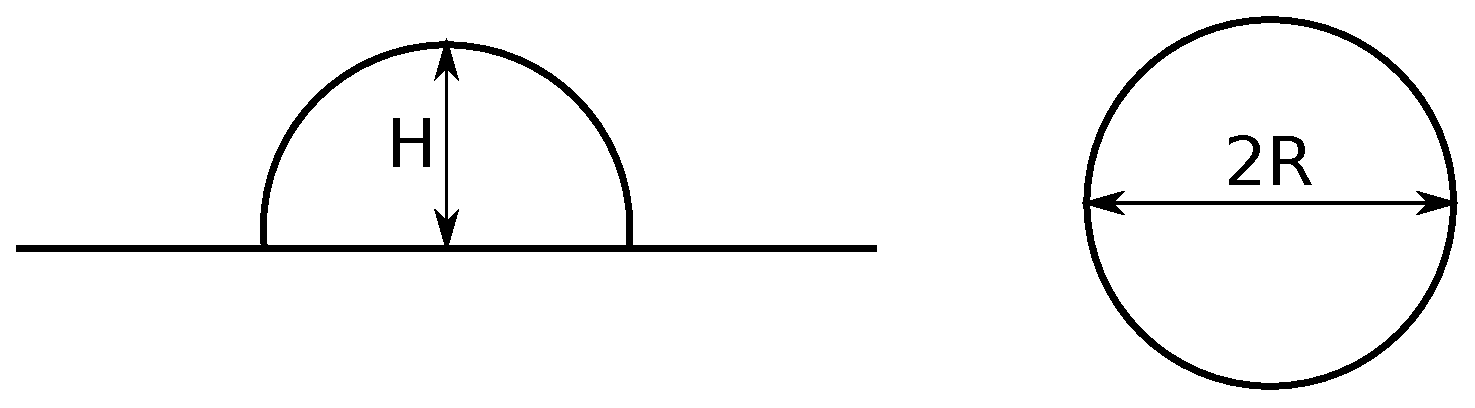
\includegraphics[width=0.6\columnwidth]{Figures/sphere}
\caption{Sketch of a (truncated) Sphere.}
\end{center}
\label{sphere}
\end{figure} 

\FloatBarrier

\paragraph{Parameters:}
\begin{itemize}
\item radius $R$,
\item height $H$.
\end{itemize}

\paragraph{Restrictions on the parameters:} $0 \leq H\leq 2R$.

\paragraph{Properties:}
\begin{itemize}
\item volume $V=\pi R^3 \left[\dfrac{2}{3} + \dfrac{H-R}{R} - \dfrac{1}{3}\left(\dfrac{H-R}{R}\right)^3\right]$,
\item particle surface seen from above $S = \left\{\begin{array}{ll} \pi R^2, & H \geq R \\
         \pi\left(2RH-H^2\right), & H < R \end{array}\right. $.
%\item gyration radius along $z$ axis %$R_g = \left\{\begin{array}{ll}
%R, & H > R \\ \sqrt{2RH-H^2}, & H < R \end{array}\right. .$
\end{itemize}

\subsection{Expression of the form factor}
\begin{equation}  
F_{\text{sphere}}(\mathbf{q},R, H)= 2\pi \exp[i q_z (H-R)]\int_{R-H} ^{R} R_z^2 \frac{J_1(q_{\parallel} R_z) }{q_{\parallel} R_z} \exp(i q_z z) dz
\label{eq:ffsphere}
\end{equation}
with $J_1(x)$ the first order
Bessel function of the first kind \cite{AbSt64}, $q_{\parallel} =
\sqrt{q_x^2+q_y^2}$, and $R_z = \sqrt{R^2-z^2}$

\paragraph{Syntax:} \Code{FormFactorSphere(radius, height)}

\subsection{Examples}
Figure~\ref{figSphereEx} shows the normalized intensity $|F|^2/V^2$, computed with $R=5$~nm and $H=7$~nm:
\begin{figure}[h]
\begin{center}
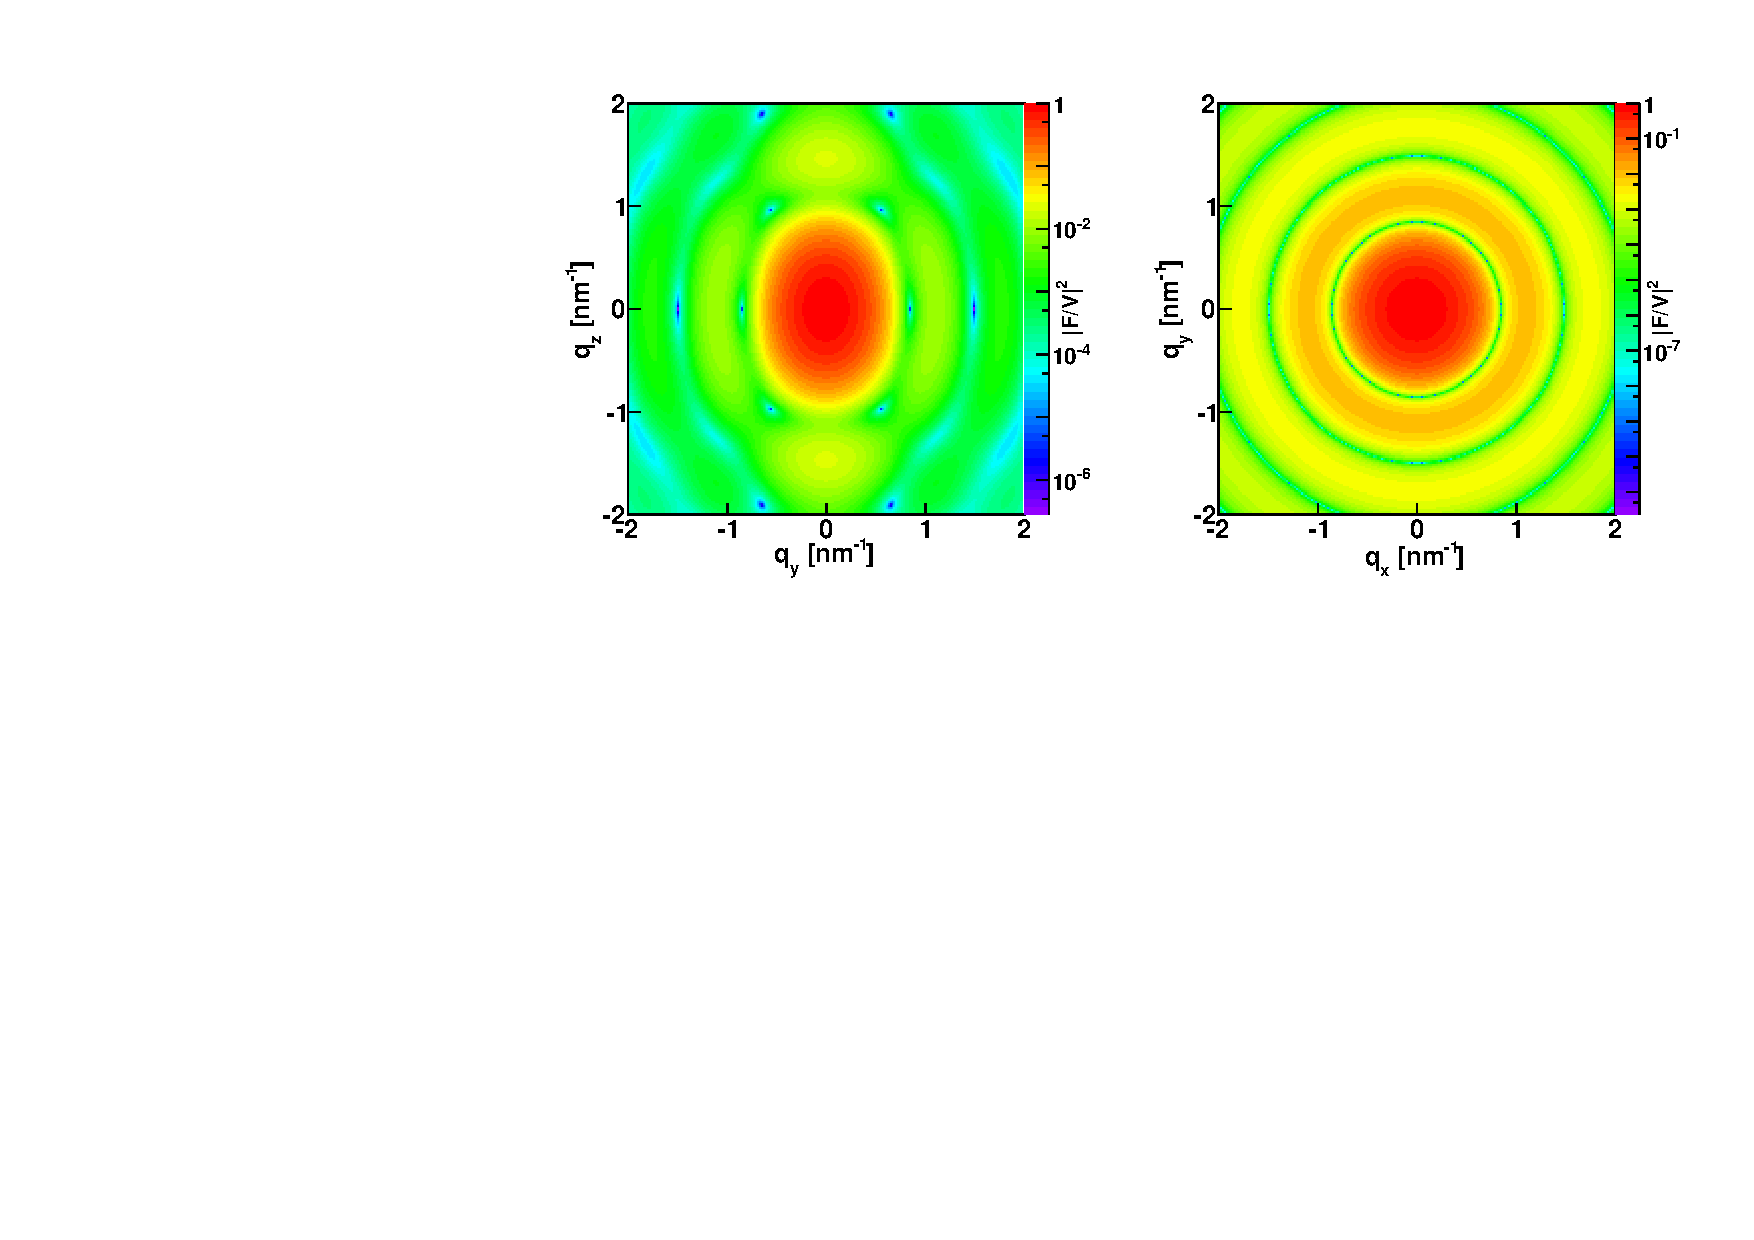
\includegraphics[width=0.9\textwidth]{Figures/figffsphere}
\end{center}
\caption{Normalized intensity for the form factor of a truncated Sphere
  $|F|^2/V^2$, plotted against ($q_z$, $q_y$) and ($q_x$, $q_y$) and
  computed with $R=5$~nm and $H=7$~nm.}
\label{figSphereEx}
\end{figure}

\FloatBarrier


\subsection{References}
Equation~(\ref{eq:ffsphere}) agrees with the \lq\lq Sphere\rq\rq ~form
factor of \IsGISAXS~\cite{Laz02}.
\newpage{\cleardoublepage}
%%%%%%%%%%%%%%%%%%%%%%%%%%%%%%%%%%%%
\section{Full spheroid} \SecLabel{FullSpheroid}  

\subsection{Real-space geometry}
A full spheroid is generated by rotating an ellipse around the vertical
axis (see fig.~\ref{fullspheroid}).

\begin{figure}[ht]
\begin{center}
%\includegraphics[width=0.6\columnwidth]{Figures/Full_Spheroid}
\caption{Sketch of a Full Spheroid. }
\end{center}
\label{fullspheroid}
\end{figure}


\paragraph{Parameters:}
\begin{itemize}
\item radius $R$,
\item height $H$.
\end{itemize}

\paragraph{Properties:}
\begin{itemize}
\item volume $V =\dfrac{2}{3}R^2H$,
\item particle surface seen from above $S =\pi R^2$. 
%\item radius of gyration
\end{itemize}

\subsection{Expression of the form factor}
\begin{equation*}
F_{\rm{FullSpheroid}}(\mathbf{q}, R, H) = 4\pi \exp(i q_z H/2) \int_0 ^{H/2}R_z ^2
\frac{J_1(q_{\parallel}R_z)}{q_{\parallel}R_z} \cos(q_z z) dz,
with 
\end{equation*}
with $J_1(x)$ the first order
Bessel function of the first kind \cite{AbSt64},
$R_z = R\sqrt{1-\frac{4z^2}{H^2}}$, $\gamma_z = \sqrt{(q_x R_z)^2+(q_y R_z)^2}$.


\paragraph{Syntax:} \Code{FormFactorFullSpheroid(radius,height)}

\subsection{Examples}
Figure~\ref{figFFfspheroidEx} shows the normalized intensity
$|F|^2/V^2$, computed with $R=10$~nm, and $H=13$~nm.
\begin{figure}[h]
\begin{center}
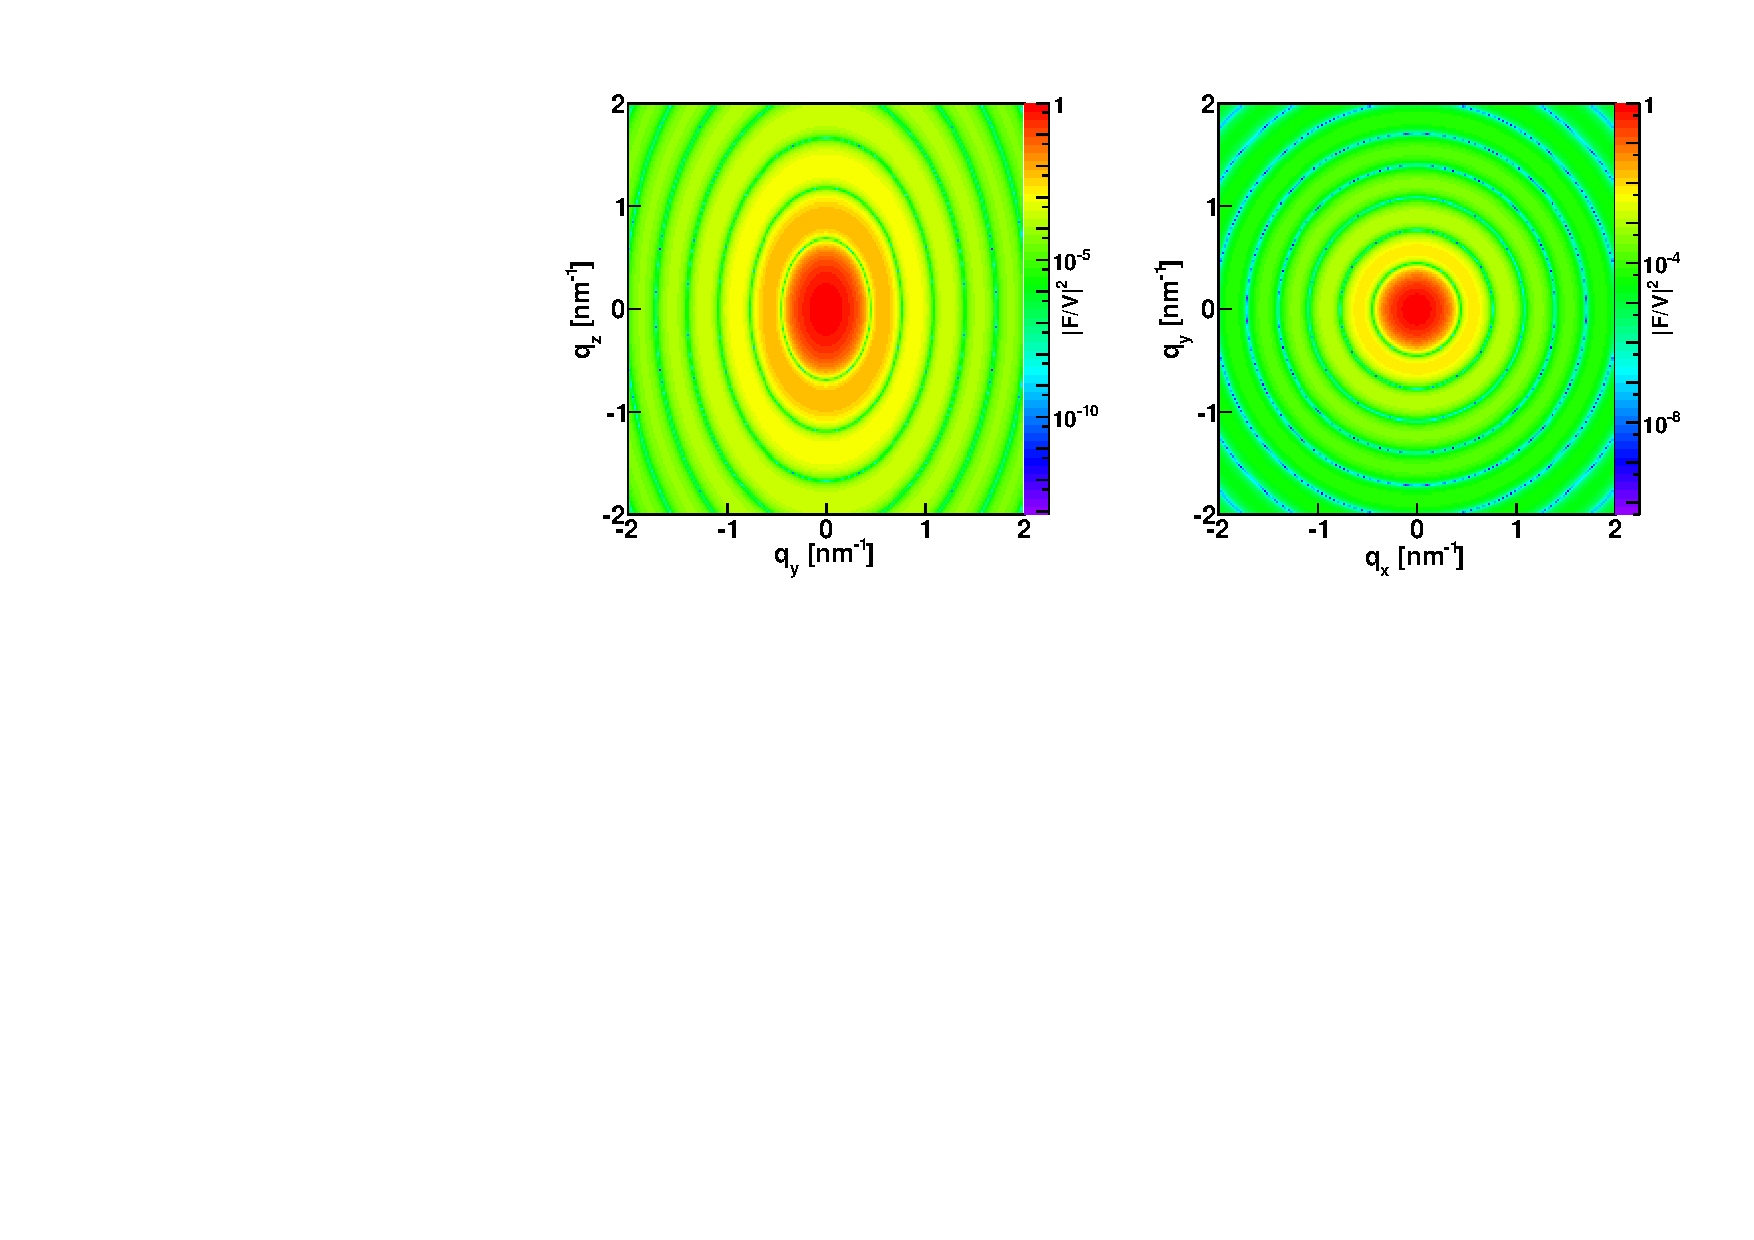
\includegraphics[width=0.9\textwidth]{Figures/figfffspheroid}
\end{center}
\caption{Normalized intensity for the form factor of a full spheroid
  $|F|^2/V^2$, plotted against ($q_z$, $q_y$) and ($q_x$, $q_y$) and
  computed with $R=10$~nm and $H=13$~nm.}
\label{figFFfspheroidEx}
\end{figure}


\subsection{References}
%The expression is identical to \Code{IsGISAXS} manual. In the code,
%the integration is over $[-H/2, H/2]$ with $\exp(iq_z z)$ instead of
%the cosine.
%In \Code{IsGISAXS}, factor 4 instead of 2 in the expression of the
%volume. In the code there is also a problem with an extra factor 2 in the function to integrate.

\newpage{\cleardoublepage}

%%%%%%%%%%%%%%%%%%%%%%%%%%%%%%%%%%%%
\section{Truncated spheroid} \SecLabel{Spheroid}

\subsection{Real-space geometry}
This shape is a spheroidal dome: a portion of a full spheroid cut off
by a plane perpendicular to the $z$-axis.

\begin{figure}[ht]
\begin{center}
%\includegraphics[width=0.6\columnwidth]{Figures/Spheroid}
\caption{Sketch of a truncated Spheroid.}
\end{center}
\label{spheroid}
\end{figure}

\paragraph{Parameters:}
\begin{itemize}
\item radius $R$,
\item height $H$,
\item height\_flattening coeeficient in the perpendicular direction $f_p$.
\end{itemize}

\paragraph{Restrictions on the parameters:} $0< \dfrac{H}{R}< 2f_p$.

\paragraph{Properties:}
\begin{itemize}
\item volume $V = \dfrac{\pi R H^2}{f_p}  \Big(1-\dfrac{H}{3f_p R}\Big)$,
\item particle surface seen from above $S = \left\{\begin{array}{ll} \pi R^2, & H \geq f_pR \\
         \pi\left(\dfrac{2RH}{f_p}-\dfrac{H^2}{f_p^2}\right), & H < R \end{array}\right.$.
%\item radius of gyration
\end{itemize}

\subsection{Expression of the form factor}
\begin{equation*}
F_{\rm{spheroid}}(\mathbf{q},R, H,f_p) =   2\pi \exp[iq_z(H-f_pR)] \int_{f_p R-H} ^{f_p R} R_z
        ^2\frac{J_1(q_{\parallel}R_z)}{q_{\parallel}R_z} \exp(i q_z z) dz
\end{equation*}
with $J_1(x)$ the first order
Bessel function of the first kind \cite{AbSt64}, $q_{\parallel}=\sqrt{q_x^2+q_y^2} $ and $R_z=\sqrt{R^2-z^2/f_p^2}$.

\paragraph{Syntax:} \Code{FormFactorSpheroid(radius, height, height\_flattening)}

\subsection{Examples}
Figure~\ref{figFFspheroidEx} shows the normalized intensity
$|F|^2/V^2$, computed with $R=7$~nm, $H=9$~nm and $f_p=1.2$.

\begin{figure}[h]
\begin{center}
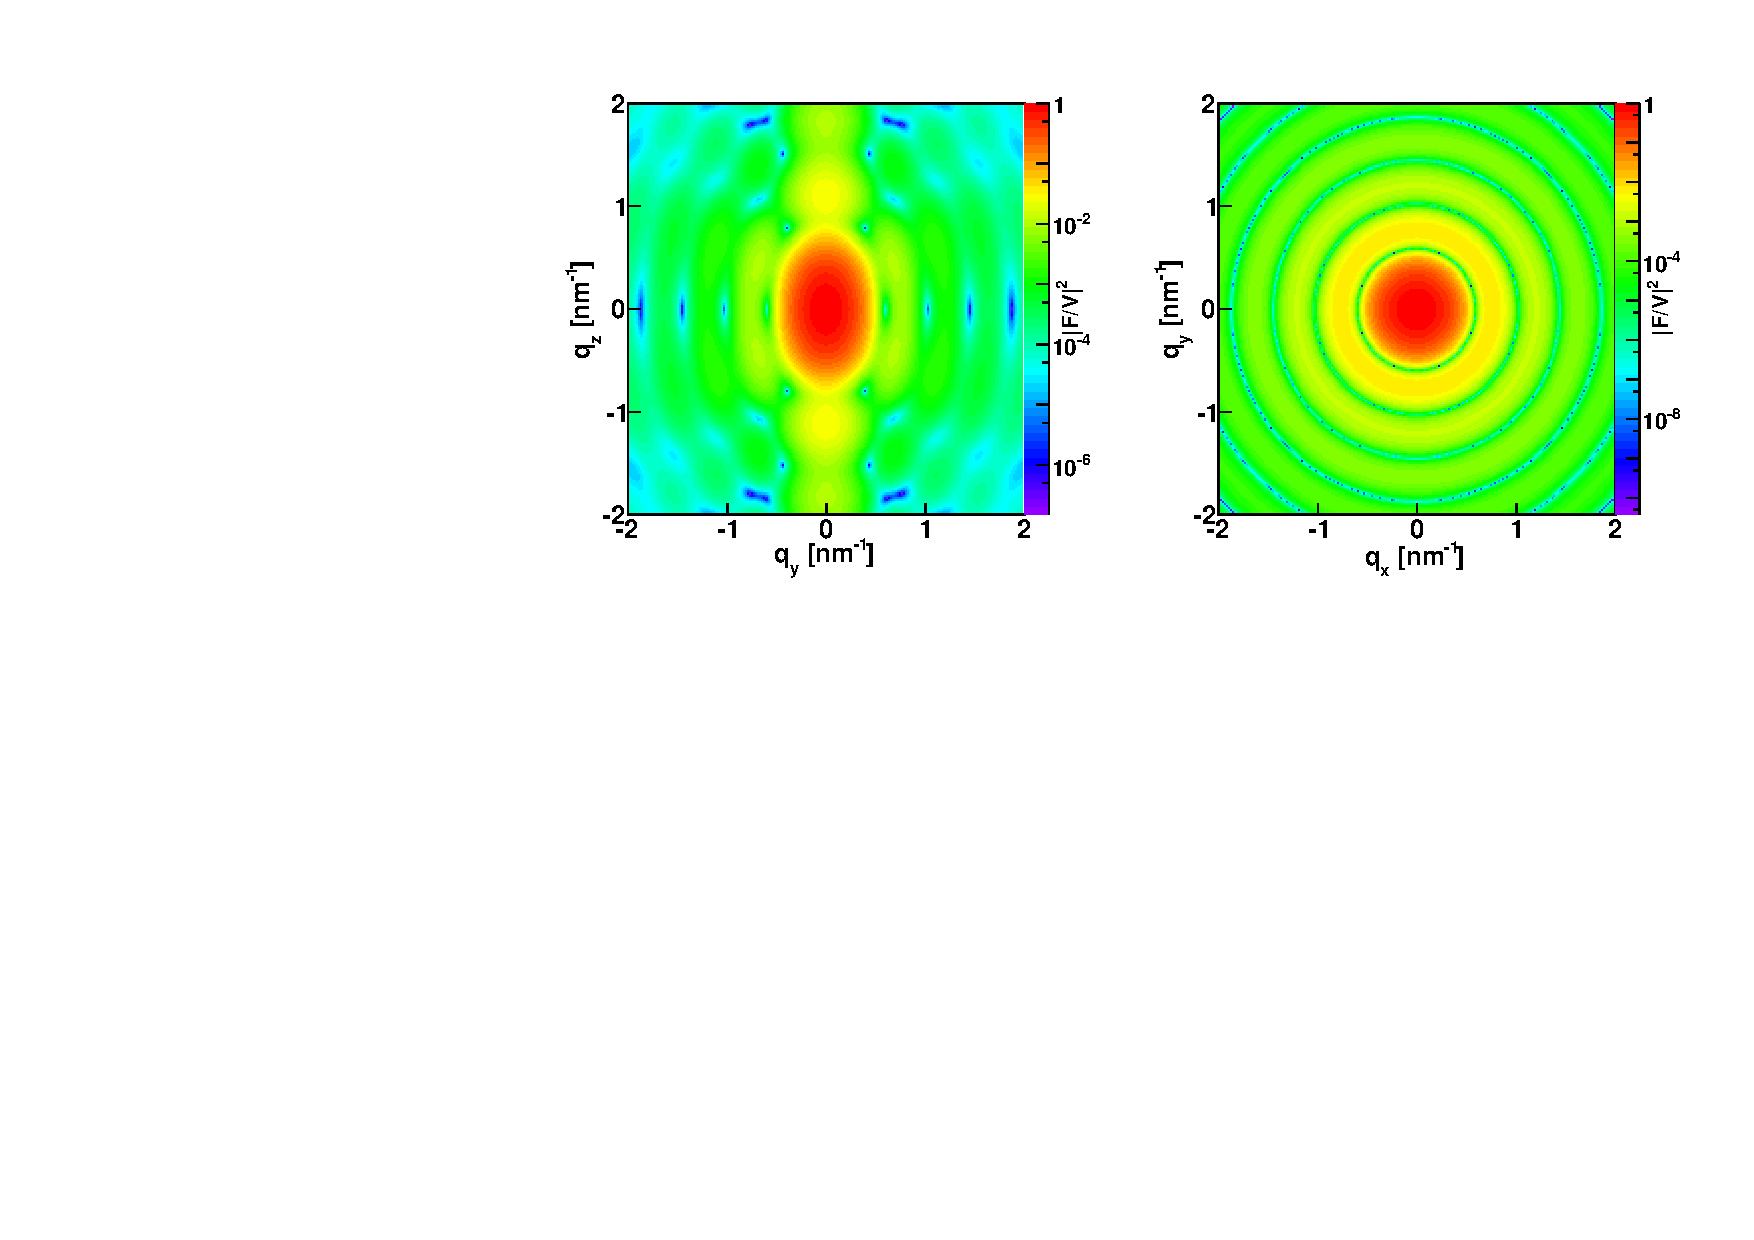
\includegraphics[width=0.9\textwidth]{Figures/figffspheroid}
\end{center}
\caption{Normalized intensity for the form factor of a truncated Spheroid
  $|F|^2/V^2$, plotted against ($q_z$, $q_y$) and ($q_x$, $q_y$) and
  computed with $R=7$~nm, $H=9$~nm, and $f_p=1.2$.}
\label{figFFspheroidEx}
\end{figure}
\FloatBarrier


\subsection{References}
%In \Code{IsGISAXS}'s manual there is an extra factor 2 in the
%expression of the volume.

\newpage{\cleardoublepage}
%%%%%%%%%%%%%%%%%%%%%%%%%%%%%%%%%%%%
\section{Hemi ellipsoid} \SecLabel{HemiEllipsoid}  

\subsection{Real-space geometry}
This shape is a truncated ellipsoid as shown in fig.~\ref{hemiellipsoid}.

\begin{figure}[ht]
\begin{center}
%\includegraphics[width=0.6\columnwidth]{Figures/Hemi-ellipsoid}
\caption{Sketch of an Hemi-ellipsoid.}
\end{center}
\label{hemiellipsoid}
\end{figure}

\paragraph{Parameters:}
\begin{itemize}
\item $r_a$ = half length of the ellipse main axis parallel to $x$,
\item$r_b$ = half length of the ellipse main axis parallel to $y$, 
\item $H$ = height (half length of the vertical main axis of a full ellipsoid).
\end{itemize}

\paragraph{Properties:}
\begin{itemize}
\item volume $V = \dfrac{2}{3}\pi r_a r_bH$,
\item particle surface seen from above $S =\pi r_a r_b$.
%\item radius of gyration
\end{itemize}

\subsection{Expression of the form factor}
\begin{equation*}
F_{\rm{hemi-ellipsoid}}(\mathbf{q},r_a,r_b,H) = 2\pi \int_0 ^{H} r_{a,z} r_{b,z}
\frac{J_1(\gamma_z)}{\gamma_z}\exp(iq_z z)dz,
\end{equation*}
with $J_1(x)$ the first order
Bessel function of the first kind \cite{AbSt64}, $r_{a,z} = r_a \sqrt{1-\left(\dfrac{z}{H} \right)^2}$, $r_{b,z} = r_b
\sqrt{1-\left(\dfrac{z}{H} \right)^2}$ and $\gamma_z =\sqrt{(q_x r_{a,z})^2+(q_y r_{b,z})^2}$.

\paragraph{Syntax:} \Code{FormFactorHemiEllipsoid($r_a$, $r_b$, height)}

\subsection{Examples}
Figure~\ref{figFFhemiellipsEx} shows the normalized intensity
$|F|^2/V^2$, computed with $r_a=10$~nm, $r_b=6$~nm and $H=8$~nm.

\begin{figure}[h]
\begin{center}
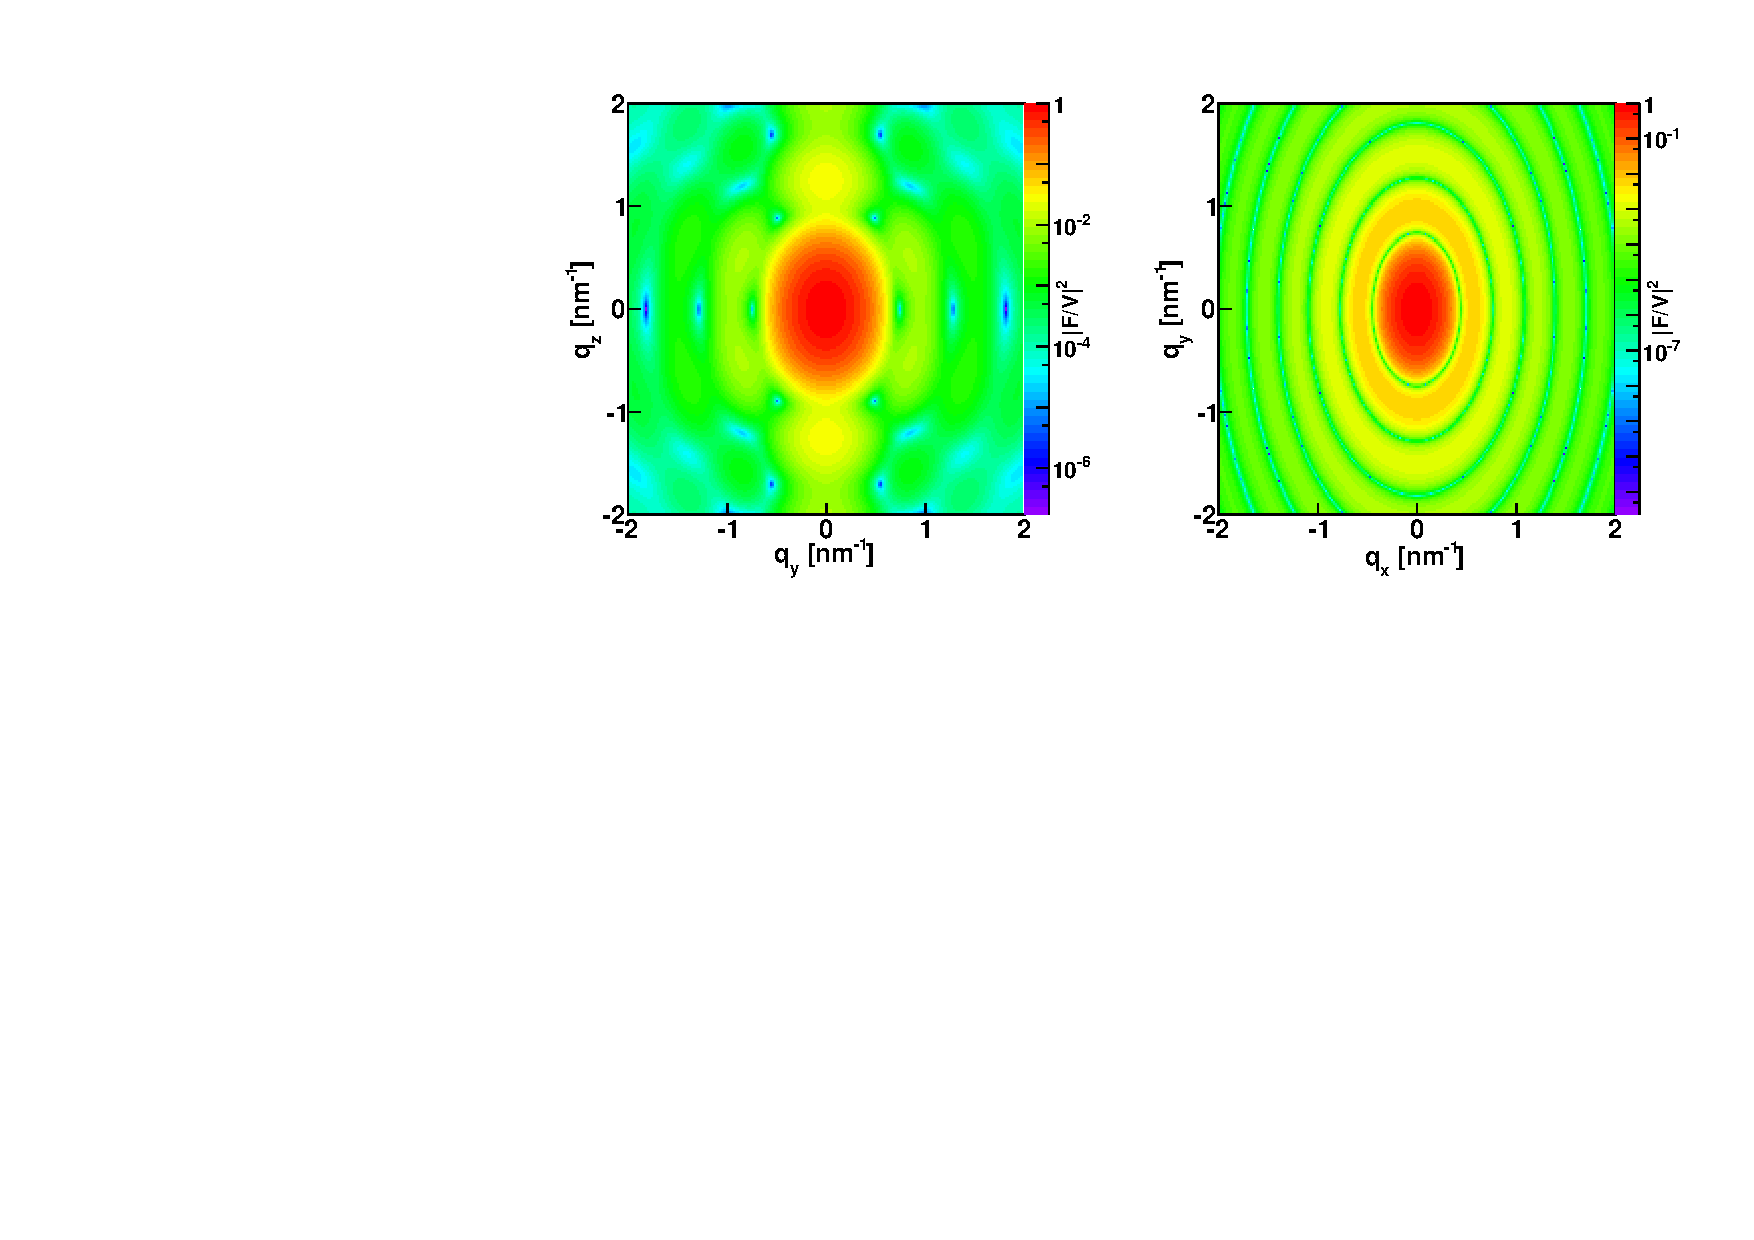
\includegraphics[width=0.9\textwidth]{Figures/figffhemiellips}
\end{center}
\caption{Normalized intensity for the form factor of an Hemi-Ellipsoid
  $|F|^2/V^2$, plotted against ($q_z$, $q_y$) and  ($q_x$, $q_y$)
  computed with $r_a=10$~nm, $r_b=6$~nm, and $H=8$~nm.}
\label{figFFhemiellipsEx}
\end{figure}
\FloatBarrier

\subsection{References}
This shape is referred to as ``Anisotropic hemi ellipsoid'' in  \Code{ISGISAXS}.
%Problem when running  \Code{ISGISAXS}.
%In \Code{IsGISAXS} manual, where does the minus sign in exp(-iq\_z z)
%come from?
\newpage{\cleardoublepage}
%%%%%%%%%%%%%%%%%%%%%%%%%%%%%%%%%%%%
\section{Ripple1} \SecLabel{Ripple1}  

\subsection{Real-space geometry}


\begin{figure}[ht]
\begin{center}
%\includegraphics[width=0.6\columnwidth]{Figures/}
\caption{Sketch}
\end{center}
\end{figure}

\paragraph{Parameters:}
\begin{itemize}
\item length 
\item width 
\item height 
\end{itemize}

\paragraph{Properties:}
\begin{itemize}
\item volume $V = $,
\item particle surface seen from above $S $.
\end{itemize}

\subsection{Expression of the form factor}

\paragraph{Syntax:} \Code{FormFactorRipple1(,,)}

\subsection{Examples}


\subsection{References}


\newpage{\cleardoublepage}
%%%%%%%%%%%%%%%%%%%%%%%%%%%%%%%%%%%%
\section{Ripple2} \SecLabel{Ripple2}  

\subsection{Real-space geometry}


\begin{figure}[ht]
\begin{center}
%\includegraphics[width=0.6\columnwidth]{Figures/}
\caption{Sketch}
\end{center}
\end{figure}

\paragraph{Parameters:}
\begin{itemize}
\item length 
\item width 
\item height 
\end{itemize}

\paragraph{Properties:}
\begin{itemize}
\item volume $V = $,
\item particle surface seen from above $S $.
\end{itemize}

\subsection{Expression of the form factor}

\paragraph{Syntax:} \Code{FormFactorRipple2(,,)}

\subsection{Examples}



\subsection{References}

